\documentclass{article}

% Language setting
% Replace `english' with e.g. `spanish' to change the document language
\usepackage[polish]{babel}
\usepackage[T1]{fontenc}
% Set page size and margins
% Replace `letterpaper' with `a4paper' for UK/EU standard size
\usepackage[a4paper,top=2cm,bottom=2cm,left=3cm,right=3cm,marginparwidth=1.75cm]{geometry}
\usepackage{url}

\usepackage[backend=biber,style=numeric]{biblatex}
\addbibresource{bibblo.bib}
% Useful packages
\usepackage{amsmath}
\usepackage{graphicx}
\usepackage{subcaption}
\usepackage{rotating}
\usepackage{geometry}
\usepackage{listings}
\usepackage{xcolor}
\usepackage{booktabs}
\usepackage{hyperref}
\usepackage{parskip}
\usepackage{lmodern}
\usepackage{hyperref}

\definecolor{codebg}{RGB}{245,245,245}
\definecolor{codeframe}{RGB}{200,200,200}
\definecolor{keyword}{RGB}{0,0,180}
\definecolor{comment}{RGB}{80,130,80}
\definecolor{string}{RGB}{160,32,32}
\definecolor{number}{RGB}{180,100,0}
\lstdefinestyle{cpp}{
	language=C++,
	backgroundcolor=\color{codebg},
	frame=single,
	rulecolor=\color{codeframe},
	basicstyle=\ttfamily\small,
	keywordstyle=\color{keyword}\bfseries,
	commentstyle=\color{comment}\itshape,
	stringstyle=\color{string},
	numberstyle=\tiny\color{gray},
	numbers=left,
	numbersep=8pt,
	tabsize=4,
	showstringspaces=false,
	breaklines=true,
	breakatwhitespace=true,
	captionpos=b,
	morekeywords={std, thread, atomic, memory_order_release},
}

\begin{document}
\begin{titlepage}

% Top logo and faculty name
\begin{center}
	\vspace*{0.5cm}
	% Pamiętaj o pliku logo.png w folderze projektu
	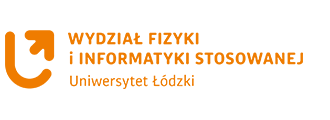
\includegraphics[width=4.69861in,height=1.55278in]{logo.png}
\end{center}

\vspace{1.2cm}

% Name line
\begin{center}
	{\fontsize{16pt}{20pt}\selectfont
		\textbf{Patryk Michalak\\[-0.2em]}}
\end{center}

\vspace{1.3cm}

% Study info block
\noindent
Kierunek: informatyka\\
Specjalno\'s\'c: informatyka stosowana\\
Specjalizacja: Algorytmy i Programowanie\\
Numer albumu: 410205\\

\vspace{2.0cm}

% Thesis title line
\begin{center}
	{\fontsize{16pt}{20pt}\selectfont
		\textbf{
			Niskopoziomowa emulacja sprzętowa implementacja architekturę systemową konsoli Game Boy\\[-0.2em]}}
\end{center}

\vspace{2.6cm}

% Right-side engineering thesis block
\hfill
\begin{minipage}[t]{0.45\textwidth}
	\raggedleft
	{\bfseries Praca in\.zynierska}\\
	wykonana pod kierunkiem\\
	\textbf{prof. dr. hab. Pawła Kowalczyka\\}
	w Katedrze Fizyki Ciała Stałego\\
	WFiIS U\L{}
\end{minipage}

\vfill

% Bottom city and year
\begin{center}
	\L{}\'od\'z 2026\\[-0.2em]
\end{center}
\end{titlepage}
\clearpage
	\tableofcontents
	\clearpage
\section{Wstęp}

\subsection{Opis problemu}

Konsola \textit{Game Boy}, wyprodukowana przez firmę \textit{Nintendo} i wprowadzona na rynek japoński 21 kwietnia 1989 roku, stała się jednym z najbardziej rozpoznawalnych urządzeń w historii elektronicznej rozrywki. Game Boy odniosła znaczący sukces komercyjny – w ciągu pierwszych lat od premiery sprzedano ponad 20 milionów egzemplarzy. W kolejnych latach konsola została wprowadzona na rynki zachodnie, gdzie również zdobyła dużą popularność. Łączna sprzedaż wszystkich wariantów urządzenia uczyniła ją jedną z najlepiej sprzedających się konsol przenośnych w historii.

Gry dla konsoli były dystrybuowane w postaci wymiennych kartridży (Game Pak), zawierających pamięć ROM z kodem programu, danymi graficznymi oraz dźwiękowymi. W niektórych przypadkach kartridże wyposażone były dodatkowo w pamięć RAM oraz baterię podtrzymującą stan gry. Architektura sprzętowa konsoli opierała się na 8-bitowym procesorze taktowanym częstotliwością około 4,19 MHz, a obraz generowany był w rozdzielczości 160×144 pikseli przy czterech poziomach szarości.

Wraz z zakończeniem produkcji konsoli przez \textit{Nintendo} dostęp do oryginalnego sprzętu stał się ograniczony. Znaczna część tytułów wydanych wyłącznie na tę platformę nie została oficjalnie przeniesiona na nowsze systemy. W konsekwencji wiele gier pozostaje dostępnych jedynie poprzez zachowane egzemplarze konsoli oraz kartridże, co utrudnia ich użytkowanie oraz archiwizację.

\subsection{Emulatory}

Jednym z rozwiązań problemu ograniczonej dostępności oryginalnego sprzętu są emulatory, czyli programy komputerowe umożliwiające odtworzenie funkcjonalności danego systemu sprzętowego w środowisku wirtualnym. Emulator odwzorowuje działanie procesora, pamięci, układów graficznych oraz urządzeń wejścia/wyjścia w sposób pozwalający na uruchamianie oryginalnego oprogramowania.

Emulatory znajdują zastosowanie nie tylko w środowisku graczy, lecz również w badaniach nad architekturą systemów komputerowych, analizie kompatybilności oprogramowania oraz cyfrowej archiwizacji dziedzictwa technologicznego. Umożliwiają one zachowanie historycznej wartości gier i systemów, które w przeciwnym razie mogłyby zostać utracone wraz z degradacją fizycznych nośników.

Wyróżnia się dwa podstawowe podejścia do emulacji:
\begin{itemize}
	\item \textbf{Emulacja pełna} – polegająca na wiernym odwzorowaniu wszystkich kluczowych komponentów sprzętowych systemu, w tym procesora, pamięci, grafiki oraz dźwięku.
	\item \textbf{Emulacja częściowa} – obejmująca jedynie wybrane elementy systemu, co może ograniczać kompatybilność z oryginalnym oprogramowaniem.
\end{itemize}

W kontekście niniejszej pracy przyjęto założenie realizacji emulacji pełnej w zakresie podstawowej funkcjonalności konsoli.

\subsection{Założenia i cel pracy}

Celem niniejszej pracy jest zaprojektowanie oraz implementacja emulatora konsoli Game Boy w języku programowania C++, z wykorzystaniem biblioteki Raylib do obsługi warstwy graficznej i wejścia użytkownika. Projekt zakłada odwzorowanie podstawowych mechanizmów działania oryginalnej architektury sprzętowej w stopniu umożliwiającym uruchamianie wybranej klasy gier.

Zakres pracy obejmuje:
\begin{itemize}
	\item implementację emulacji procesora oraz mapy pamięci konsoli,
	\item odwzorowanie mechanizmu wyświetlania obrazu,
	\item obsługę wejścia użytkownika z wykorzystaniem klawiatury,
	\item możliwość wczytywania obrazów ROM typu \textit{ROM Only},
	\item zapewnienie wieloplatformowości (Windows, Linux, macOS).
\end{itemize}

W ramach projektu przyjęto ograniczenie do obsługi podstawowego typu kartridża zawierającego wyłącznie pamięć ROM, bez dodatkowych kontrolerów pamięci (MBC). Emulator przeznaczony jest do uruchamiania cyfrowych kopii gier pozyskanych przez użytkownika z posiadanych nośników.

Poprawność działania systemu zostanie zweryfikowana poprzez porównanie wyników emulacji z publicznie dostępnymi testami zgodności opracowanymi przez społeczność dokumentującą architekturę konsoli.
%
\subsection{Grupa docelowa}

Odbiorcami opracowanego systemu są użytkownicy posiadający legalne kopie gier przeznaczonych na konsolę Game Boy, zainteresowani ich uruchamianiem na współczesnych komputerach osobistych. Emulator może stanowić również narzędzie edukacyjne dla osób zainteresowanych architekturą systemów wbudowanych oraz mechanizmami niskopoziomowego działania sprzętu.

\subsection{Inne emulatory Game Boya}

Na przestrzeni lat powstało wiele emulatorów Game Boya o różnym stopniu
dokładności, przenośności i przeznaczeniu. Poniżej opisano najważniejsze
projekty open source, które stanowią punkt odniesienia dla współczesnych
implementacji.

\paragraph{SameBoy}
\texttt{SameBoy}~\cite{sameboy} jest jednym z najbardziej dokładnych
dostępnych emulatorów Game Boya i Game Boya Color. Projekt jest
wieloplatformowy -- obsługuje systemy macOS, Windows oraz platformy
uniksopodobne. Oprócz wysokiej wierności emulacji sprzętu, \texttt{SameBoy}
oferuje rozbudowane narzędzia diagnostyczne oraz emulację akcesoriów,
takich jak Game Boy Camera i Game Boy Printer.

\paragraph{mGBA}
\texttt{mGBA}~\cite{mgba} to wieloplatformowy emulator Game Boya Advance,
obsługujący również Game Boya i Game Boya Color. Projekt kładzie nacisk
zarówno na szybkość działania, jak i na dokładność emulacji. Emulator
dostępny jest na systemy Windows, macOS, Linux, a także jako homebrew na
konsole Nintendo Switch, Wii oraz PlayStation Vita. \texttt{mGBA} wspiera
skryptowanie w języku Lua, co czyni go popularnym narzędziem wśród
twórców narzędzi pomocniczych i speedrunnerów.

\paragraph{Gearboy}
\texttt{Gearboy}~\cite{gearboy} to wieloplatformowy emulator Game Boya
i Game Boya Color napisany w C++. Projekt wyróżnia się dokładną emulacją
procesora i kontrolera LCD, przechodzi testy \texttt{cpu\_instrs.gb} oraz
\texttt{instr\_timing.gb} autorstwa Blarrga. Emulator posiada rozbudowany
debugger z deasemblerem, punktami przerwań oraz inspektorem pamięci VRAM.

\paragraph{VisualBoyAdvance-M}
\texttt{VisualBoyAdvance-M}~\cite{vba} jest następcą oryginalnego emulatora
\texttt{VisualBoyAdvance} i obsługuje Game Boya, Game Boya Color oraz Game
Boya Advance. Projekt dostępny jest na systemy Windows, macOS, Linux oraz
Android. Emulator wspiera popularne systemy kodów cheat, takie jak
GameShark i CodeBreaker.
\newpage
\section{Analiza architektury systemowej konsoli Game Boy}
\subsection{Specyfikacja techniczna}
Zespół \textit{Nintendo Research And Development 1}, pod przewodnictwem Gunpei Yokoi i Satoru Okady, zaprojektował 8-bitową konsolę Game Boy. Charakteryzuje się wyświetlaczem matrycowym o rozdzielczości 160x144 pikseli, D-padem, czterema przyciskami gry i jednym głośnikiem. Używa stworzonych na potrzebe konsoli kartridże \textit{GamePak}. Zasilana była przez 4 baterie AA. Gracze mogli korzystać z kabla Game Link Cable do połączenia dwóch Game Boyów dla rozgrywki wieloosobowej bądź transferu danych dla wspierających gier. Chociaż wyświetlacz monochromatyczny był gorszy niż u konkurencji, utrzymanie konsoli w jednym kolorze przyczyniło się do większonej żywotności i wymaganej liczbie baterii.  \cite{wikipedia-gameboy}. 
\subsection{Procesor i SoC}
Procesorem Gameboya był specjalnie wytworzyny na potrzeby konsoli  8-bitowy procesor SM83 firmy Sharp. \cite{gbctr}. Procesor był wzorowany na dwóch innych procesorach- 8080 firmy Intel i Z80 firmy Zilog. Procesor znajdował się na płytce wraz innymi komponentami takimi jak pamięć RAM i ROM. Cała płytka jest określana jako SoC (System on Chip) i oryginalny Game Boy zawierał DMG-CPU znany także jako Sharp LR35902 \cite{copetti}. SoC był wpinany do płyty głównej, która zawierała dodatkową pamięć RAM i Video RAM (VRAM) . Płyta główna łączyła także inne kompomenty jak ekran, głośnik czy kontroler.

Procesor zawiera osiem 8-bitowych rejestrów: A,B,C,D,E,F,H,L. Rejestry mogą łączyć się w 16-bitowe rejestry: AF, BC, DE, HL. Rejestr F jest używany jako flagi procesora w wypadku operacji arymetycznych:
\begin{itemize}
	\item Bit 7 - Zero (Z), jeśli operacja zwróciła zero,
	\item Bit 6 -  Negacja (N), używana gdy ostatnia operacją była porównaniem bądź odejmowaniem,
	\item Bit 5 - Half Carry (H), jeśli doszło do przesunięcia na bicie 3,
	\item Bit 4 - Carry (C), jeśli doszło do przesunięcia na bicie 7.
\end{itemize} 
Bity od 3 do 0 są nieużywane i zawsze powinny być zerowane. Rejestr A jest używany jako akumulator w operacja arytmetcznych.
\subsubsection{Model czasowy systemu}

Działanie konsoli Game Boy oparte jest na synchronicznym modelu czasowym, w którym wszystkie główne komponenty systemu --- procesor, układ graficzny oraz timery sprzętowe --- pracują w oparciu o wspólne źródło taktowania. Nominalna częstotliwość zegara systemowego wynosi $4{,}194304$~MHz, co determinuje tempo wykonywania instrukcji procesora oraz przebieg cykli pracy pozostałych bloków funkcjonalnych.

\paragraph{Cykle maszynowe procesora}

Procesor wykonuje instrukcje w jednostkach zwanych cyklami maszynowymi (ang. \emph{machine cycles}), z których każdy obejmuje określoną liczbę taktów zegara systemowego. Czas wykonania instrukcji zależy od jej złożoności i wynosi zazwyczaj od jednego do kilku cykli maszynowych. Model czasowy procesora ma charakter deterministyczny, co oznacza, że liczba cykli wymaganych do wykonania danej instrukcji jest stała i niezależna od kontekstu wykonania.

\paragraph{Synchronizacja z układem graficznym}

Układ graficzny pracuje równolegle z procesorem i cyklicznie przechodzi przez zdefiniowane fazy generowania obrazu. Każda ramka obrazu składa się z sekwencji linii skanowania, a przebieg ich przetwarzania wyznacza rytm pracy całego systemu. W określonych fazach generowania obrazu dostęp procesora do wybranych obszarów pamięci wideo jest ograniczony, co stanowi bezpośrednią konsekwencję współdzielenia zasobów pamięci pomiędzy jednostkami systemu.

\paragraph{System timerów sprzętowych}

Konsola wyposażona jest w sprzętowe układy odmierzania czasu, których działanie jest bezpośrednio powiązane z zegarem systemowym. Timery te generują zdarzenia okresowe wykorzystywane do synchronizacji logiki programu, pomiaru czasu oraz inicjowania przerwań sprzętowych. Ich konfiguracja pozwala na wybór różnych częstotliwości zliczania poprzez dzielenie sygnału zegarowego.




\subsection{Zestaw Instrukcji}

Zestaw Rozkazów (instruction set architecture, ISA) (rysunek \ref{fig:op_tables} i rysunek \ref{fig:op_tables_cb}) stanowi rozwinięcie koncepcji znanych z mikroprocesorów rodziny Z80, z licznymi uproszczeniami i modyfikacjami dostosowanymi do zastosowań w systemie przenośnym. Wszytkie rozkazy można systematycznie sklasyfikować na poszczególne grupy.

Każda instrukcja zapisywana jest w formie kodu binarnego (opcode) od rozmiarze 1 bajtów (2 w przypadku gdy pierwszy bajt to \text{0xCB}). Tabela pokazująca tworzenie kodów binarnych dla części instrukcji  pokazana jest na rysunku \ref{fig:op_tables}, gdzie na rysunku \ref{fig:op_tables_cb} są przedstowione wszytkie instrukcje z przedrostkiem \text{CB}. W szczególności aby utworzyć kod dla \text{OR A, H} od opcodzie równym \text{0x} starsza, 4 bitowa cześć kodu binarnego wybierana jest z odpowiedniego wiersza i w omawianym tu przypadku wynosi B, gdzie młodsze bity kodują kolumnę 4. Wybrana instrukcja jest zaznaczona na rysunku \ref{fig:op_tables}

Instrukcje tej grupy odpowiadają za przemieszczanie informacji pomiędzy rejestrami, pamięcią oraz natychmiastowymi wartościami liczbowymi. Do najważniejszych operacji należą:
\begin{sidewaysfigure}
	\centering
	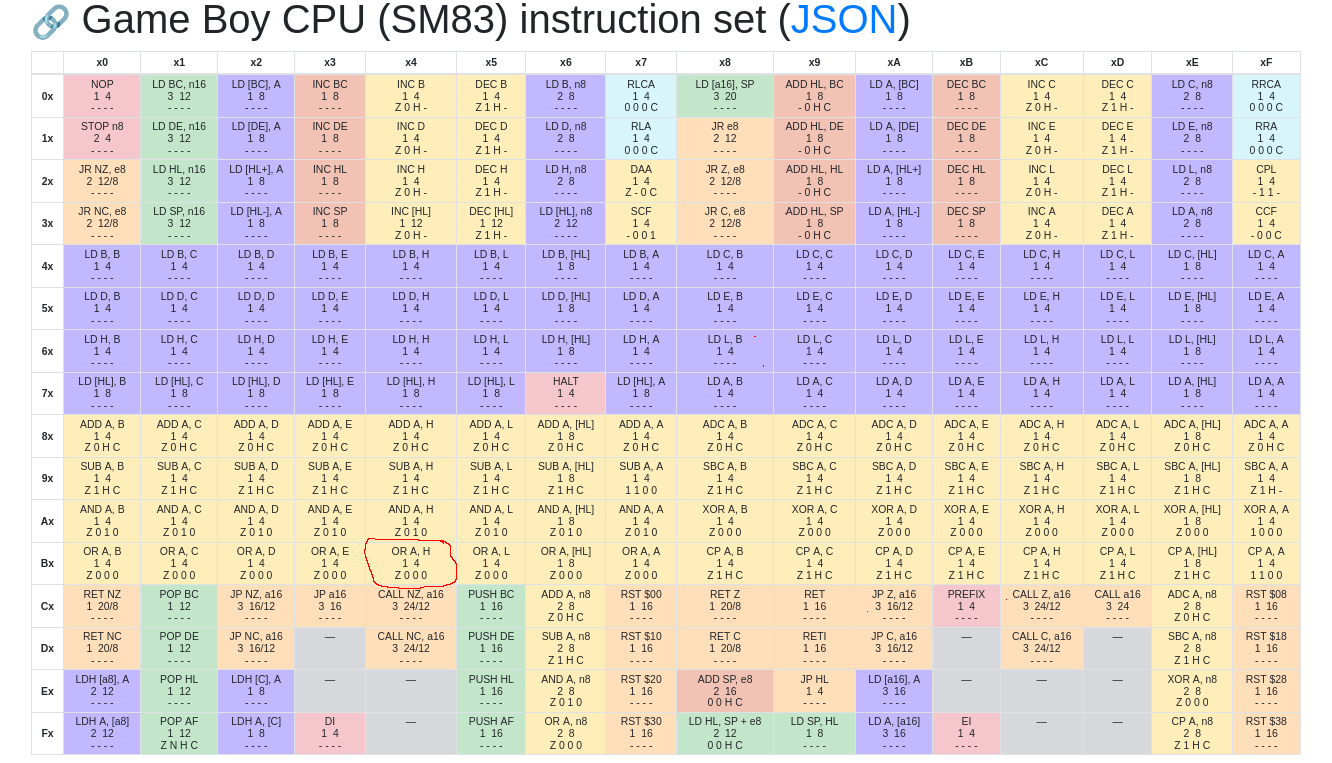
\includegraphics[width=\textheight]{gbobtables.png}
	\caption{Tablica rozmieszczenia instrukcji procesora SM83. Źródło: \cite{opcodes}}
	\label{fig:op_tables}
\end{sidewaysfigure}

\begin{sidewaysfigure}
	\centering
	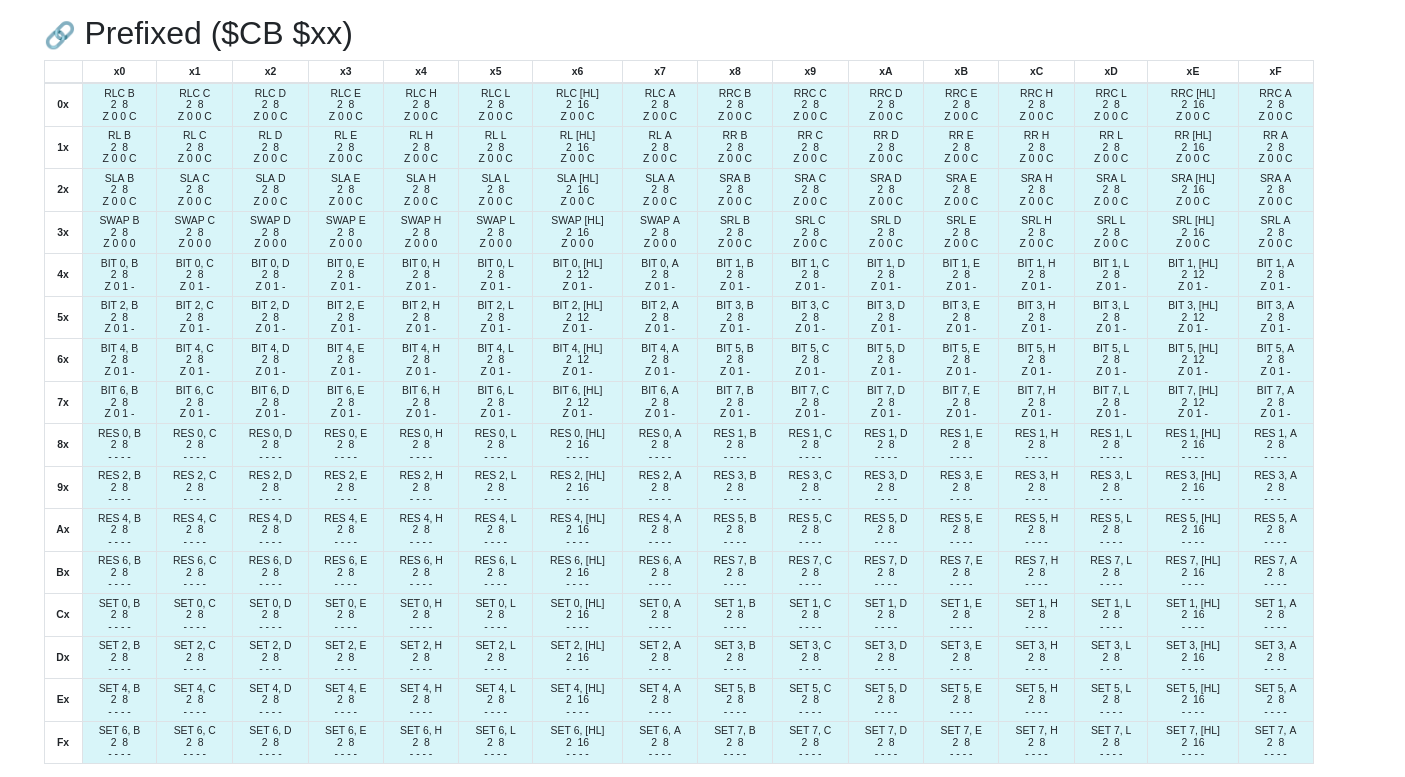
\includegraphics[width=\textheight]{gbobtables_cb.png}
	\caption{Tablica rozmieszczenia instrukcji po opcodzie 0xCB procesora SM83. Źródło: \cite{opcodes}}
	\label{fig:op_tables_cb}
\end{sidewaysfigure}

\subsubsection{Instrukcje transferu danych}

\begin{itemize}
	\item \textbf{LD (Load)} -- realizuje kopiowanie danych pomiędzy rejestrami ogólnego przeznaczenia (A, B, C, D, E, H, L), parami rejestrów oraz komórkami pamięci adresowanymi bezpośrednio lub pośrednio.
	\item \textbf{LDH} -- specjalizowana forma transferu do i z obszaru pamięci o wysokim adresie (High RAM).
	\item \textbf{PUSH / POP} -- zapis i odczyt danych na stosie, z wykorzystaniem wskaźnika stosu SP.
\end{itemize}

Instrukcje transferu nie modyfikują danych źródłowych (z wyjątkiem operacji wykonywanych na stosie), a ich podstawową funkcją jest reorganizacja informacji w przestrzeni rejestrowo-pamięciowej procesora.

\subsubsection{Instrukcje arytmetyczne}

Instrukcje arytmetyczne realizują operacje matematyczne na liczbach całkowitych. W SM83 operacje te wykonywane są głównie na akumulatorze A. Do kluczowych operacji należą:

\begin{itemize}
	\item \textbf{ADD / ADC} -- dodawanie bez i z uwzględnieniem flagi przeniesienia,
	\item \textbf{SUB / SBC} -- odejmowanie bez i z uwzględnieniem przeniesienia,
	\item \textbf{INC / DEC} -- inkrementacja i dekrementacja rejestrów oraz komórek pamięci,
	\item \textbf{DAA} -- korekcja wyniku dodawania do postaci BCD,
	\item \textbf{CP} -- porównanie wartości bez zapisu wyniku (modyfikowane są jedynie flagi).
\end{itemize}

Instrukcje te aktualizują rejestr flag (Z, N, H, C), który odzwierciedla właściwości wyniku operacji.

\subsubsection{Instrukcje logiczne i bitowe}

Grupa ta obejmuje operacje algebry Boole’a oraz manipulacje pojedynczymi bitami. Do najważniejszych należą:

\begin{itemize}
	\item \textbf{AND, OR, XOR} -- operacje logiczne na akumulatorze,
	\item \textbf{CPL} -- negacja bitowa zawartości akumulatora,
	\item \textbf{BIT} -- test wybranego bitu,
	\item \textbf{SET / RES} -- ustawienie lub wyzerowanie wskazanego bitu.
\end{itemize}

Instrukcje bitowe umożliwiają precyzyjną kontrolę struktur danych, co jest szczególnie istotne w systemach o ograniczonych zasobach pamięci.

\subsubsection{Instrukcje przesunięć i rotacji}

Operacje tej kategorii realizują przesunięcia bitowe oraz rotacje z lub bez udziału flagi przeniesienia:

\begin{itemize}
\item \textbf{RL, RR} – rotacja w lewo/prawo przez flagę przeniesienia (CY) – bit wypchnięty z rejestru trafia do flagi, a poprzednia wartość flagi wchodzi z drugiej strony,
\item \textbf{RLC, RRC} – rotacja w lewo/prawo bez udziału flagi przeniesienia – bit wypchnięty wraca na przeciwny koniec rejestru (flaga CY jest jedynie aktualizowana, nie bierze udziału w rotacji),
\item \textbf{SLA} (Shift Left Arithmetic) – przesuwa bity w lewo. Bit 7 (najstarszy) wypychany jest do flagi CY, a na miejsce bitu 0 wstawiany jest zero. Efekt: mnożenie przez 2.
\item \textbf{SRA} (Shift Right Arithmetic) – przesuwa bity w prawo. Bit 0 (najmłodszy) wypychany jest do flagi CY, a bit 7 zachowuje swoją poprzednią wartość (zachowany jest bit znaku). Efekt: dzielenie przez 2 z zachowaniem znaku liczby ujemnej.
\item \textbf{SRL} (Shift Right Logical) – przesuwa bity w prawo. Bit 0 wypychany jest do flagi CY, a na miejsce bitu 7 wstawiany jest zero (bez względu na znak). Efekt: dzielenie przez 2 dla liczb bez znaku.
	\item \textbf{SWAP} -- zamiana półbajtów w rejestrze.
\end{itemize}

Instrukcje te są użyteczne zarówno w obliczeniach arytmetycznych, jak i w przetwarzaniu danych binarnych.

\subsubsection{Instrukcje sterowania przepływem programu}

Instrukcje sterujące odpowiadają za zmianę kolejności wykonywania programu:

\begin{itemize}
	\item \textbf{JP} -- skok bezwarunkowy lub warunkowy, gdzie warunek jest zależny od kodu operacyjnego.
	\item \textbf{JR} -- skok względny o ograniczonym zasięgu  (Między -128 a +127),
	\item \textbf{CALL / RET} -- wywołanie i powrót z podprogramu,
	\item \textbf{RST} -- szybkie wywołanie procedury o stałym adresie - często używane w procedurach o dużej uwadze czasowej (obsługa przewań)
\end{itemize}

Warunkowość operacji zależy od stanu flag procesora, co umożliwia implementację struktur decyzyjnych.

Do tej grupy należą instrukcje wpływające na stan globalny procesora:

\begin{itemize}
	\item \textbf{NOP} -- brak operacji,
	\item \textbf{HALT} -- zatrzymanie pracy CPU do momentu wystąpienia przerwania,
	\item \textbf{STOP} -- tryb niskiego poboru energii,
	\item \textbf{DI / EI} -- dezaktywacja i aktywacja systemu przerwań,
	\item \textbf{SCF / CCF} -- ustawanie i kasowanie flagi przeniesienia.
\end{itemize}

Instrukcje te mają kluczowe znaczenie dla zarządzania energią oraz obsługi zdarzeń asynchronicznych.


\subsection{Mapowanie pamięci w konsoli Game Boy}

Architektura pamięci konsoli Game Boy oparta jest na 16-bitowej przestrzeni adresowej o rozmiarze $2^{16} = 65\,536$ bajtów (64~KB). Procesor systemu, zgodny z modyfikowaną architekturą Sharp LR35902, wykorzystuje jednolitą przestrzeń adresową, w której różne zakresy adresów są przypisane do odmiennych typów pamięci oraz rejestrów sprzętowych. Taki model organizacji pamięci określany jest jako \emph{memory-mapped I/O} i umożliwia bezpośrednią komunikację procesora z układami peryferyjnymi poprzez operacje odczytu i zapisu w odpowiednich obszarach adresowych.

\subsubsection{Ogólny układ przestrzeni adresowej}

Przestrzeń adresowa Game Boya podzielona jest na segmenty o ustalonej funkcji sprzętowej. Tabela~\ref{tab:gb_memory_map} przedstawia standardowy schemat mapowania pamięci.

\begin{table}[h]
	\centering
	\begin{tabular}{lll}
		\hline
		Zakres adresów & Rozmiar & Przeznaczenie \\
		\hline
		\texttt{0000--3FFF} & 16 KB & Stała pamięć ROM banku 0 \\
		\texttt{4000--7FFF} & 16 KB & Przełączalny bank ROM \\
		\texttt{8000--9FFF} & 8 KB  & Pamięć wideo (VRAM) \\
		\texttt{A000--BFFF} & 8 KB  & Zewnętrzna pamięć RAM w kartridżu \\
		\texttt{C000--CFFF} & 4 KB  & Wewnętrzna pamięć robocza (WRAM bank 0) \\
		\texttt{D000--DFFF} & 4 KB  & Wewnętrzna pamięć robocza (bank przełączalny) \\
		\texttt{E000--FDFF} & 7.5 KB & Obszar echo pamięci WRAM \\
		\texttt{FE00--FE9F} & 160 B & Pamięć atrybutów obiektów (OAM) \\
		\texttt{FEA0--FEFF} & 96 B  & Obszar niedostępny \\
		\texttt{FF00--FF7F} & 128 B & Rejestry wejścia/wyjścia \\
		\texttt{FF80--FFFE} & 127 B & Pamięć szybka (HRAM) \\
		\texttt{FFFF}       & 1 B   & Rejestr przerwań (IE) \\
		\hline
	\end{tabular}
	\caption{Mapa pamięci konsoli Game Boy \cite{pandocs}}
	\label{tab:gb_memory_map}
\end{table}

\subsubsection{Pamięć programu i bankowanie ROM}

Dolne 32~KB przestrzeni adresowej przeznaczone jest na pamięć tylko do odczytu (ROM) zawartą w kartridżu. Pierwsze 16~KB (\texttt{0000--3FFF}) stanowi bank stały, natomiast zakres \texttt{4000--7FFF} obsługuje mechanizm przełączania banków pamięci, realizowany przez kontroler MBC (Memory Bank Controller). Dzięki temu możliwe jest adresowanie programów o rozmiarze znacznie przekraczającym 64~KB.

\subsubsection{Pamięć wideo}

Obszar \texttt{8000--9FFF} odpowiada pamięci VRAM, wykorzystywanej przez układ graficzny do przechowywania danych kafelków graficznych oraz map tła. Dostęp do tej pamięci jest ograniczony w określonych fazach cyklu wyświetlania obrazu, co wynika z synchronizacji procesora z kontrolerem LCD.

\subsubsection{Pamięć robocza i obszar echo}

Wewnętrzna pamięć robocza WRAM zajmuje zakres \texttt{C000--DFFF}. Dodatkowo obszar \texttt{E000--FDFF} stanowi tzw. echo WRAM, czyli lustrzane odwzorowanie części pamięci roboczej. Jego obecność wynika z uproszczeń sprzętowych i nie jest zalecana do programowego wykorzystania.

\subsubsection{Mapowanie urządzeń wejścia/wyjścia}

Zakres \texttt{FF00--FF7F} zawiera rejestry sterujące sprzętem, w tym kontrolerem dźwięku, systemem przerwań, timerami oraz interfejsem wejściowym. Operacje zapisu i odczytu w tych adresach odpowiadają bezpośrednim operacjom na urządzeniach peryferyjnych.

\subsubsection{Pamięć wysokiej prędkości}

Obszar \texttt{FF80--FFFE}, określany jako HRAM (High RAM), to niewielki fragment szybkiej pamięci roboczej o krótkim czasie dostępu. Ze względu na swoje właściwości jest on często wykorzystywany do przechowywania zmiennych o krytycznym znaczeniu czasowym.

\subsection{System przerwań w konsoli Game Boy}

System przerwań w konsoli Game Boy realizuje mechanizm asynchronicznej obsługi zdarzeń sprzętowych, umożliwiając procesorowi reagowanie na zdarzenia wewnętrzne i zewnętrzne bez konieczności ciągłego odpytywania urządzeń peryferyjnych. Architektura ta stanowi kluczowy element synchronizacji pracy jednostki centralnej z układami graficznymi, licznikami czasu oraz interfejsem wejściowym.

\subsubsection{Źródła przerwań}

Konsola Game Boy obsługuje pięć podstawowych źródeł przerwań sprzętowych. Każdemu z nich przypisany jest odrębny wektor przerwania oraz odpowiedni bit w rejestrach sterujących. Zestaw źródeł przerwań przedstawiono w tabeli~\ref{tab:gb_interrupts}.

\begin{table}[h]
	\centering
	\begin{tabular}{lll}
		\hline
		Bit & Nazwa przerwania & Funkcja \\
		\hline
		0 & V-Blank & Zakończenie rysowania ramki obrazu \\
		1 & LCD STAT & Zdarzenia kontrolera LCD \\
		2 & Timer & Przepełnienie timera systemowego \\
		3 & Serial & Zakończenie transmisji szeregowej \\
		4 & Joypad & Zmiana stanu kontrolera wejściowego \\
		\hline
	\end{tabular}
	\caption{Źródła przerwań w konsoli Game Boy\cite{pandocs}}
	\label{tab:gb_interrupts}
\end{table}

Przerwanie V-Blank pełni szczególną rolę, ponieważ wyznacza bezpieczny moment aktualizacji pamięci wideo. Przerwanie LCD STAT umożliwia reakcję na szczegółowe stany pracy kontrolera wyświetlania, natomiast przerwanie timera wykorzystywane jest do odmierzania czasu oraz synchronizacji logiki programu.

Pozostałe przerwania w systemie Game Boy pochodzą z kontrolera wejścia oraz interfejsu komunikacyjnego. Przerwanie wejścia (Joypad) generowane jest w momencie zmiany stanu przycisków kontrolera, co umożliwia natychmiastową reakcję programu na działania użytkownika. Z kolei przerwanie interfejsu szeregowego (Serial) wyzwalane jest po zakończeniu transmisji danych pomiędzy konsolą a urządzeniem zewnętrznym, na przykład drugą konsolą Game Boy połączoną za pomocą kabla komunikacyjnego.

\subsubsection{Rejestry sterujące systemem przerwań}

Obsługa przerwań realizowana jest poprzez dwa rejestry mapowane w przestrzeni adresowej:

\begin{itemize}
	\item \texttt{IE} (Interrupt Enable, adres \texttt{FFFF}) --- określa, które źródła przerwań są aktywne.
	\item \texttt{IF} (Interrupt Flag, adres \texttt{FF0F}) --- przechowuje informację o zgłoszonych przerwaniach.
\end{itemize}

Każdy bit w obu rejestrach odpowiada jednemu źródłu przerwania. Zgłoszenie przerwania polega na ustawieniu odpowiedniego bitu w rejestrze \texttt{IF}. Jeżeli odpowiadający mu bit w rejestrze \texttt{IE} jest ustawiony oraz globalna obsługa przerwań jest włączona, procesor inicjuje procedurę obsługi przerwania.

\subsubsection{Mechanizm obsługi przerwania}

Po wykryciu aktywnego przerwania procesor wykonuje następującą sekwencję działań:

\begin{enumerate}
	\item zakończenie bieżącej instrukcji,
	\item zapis aktualnej wartości licznika programu na stosie,
	\item wyłączenie globalnej obsługi przerwań,
	\item skok pod adres wektora przerwania.
\end{enumerate}

Adresy wektorów przerwań są stałe i przypisane do konkretnych źródeł zdarzeń. Po zakończeniu procedury obsługi przerwania wykonywana jest instrukcja powrotu, która przywraca poprzedni stan wykonania programu.

\subsubsection{Priorytety przerwań}

W przypadku jednoczesnego zgłoszenia wielu przerwań stosowany jest ustalony porządek priorytetów. Najwyższy priorytet posiada przerwanie V-Blank, a najniższy przerwanie kontrolera wejściowego. Taki schemat zapewnia deterministyczną obsługę zdarzeń związanych z generowaniem obrazu, które są krytyczne dla poprawnego działania systemu.

\subsubsection{Rola systemu przerwań w architekturze konsoli}

System przerwań stanowi podstawowy mechanizm synchronizacji komponentów sprzętowych konsoli Game Boy. Dzięki niemu możliwe jest efektywne współdziałanie procesora z kontrolerem graficznym, licznikami czasu oraz urządzeniami wejścia/wyjścia przy zachowaniu deterministycznego modelu wykonania programu. Mechanizm ten ma istotne znaczenie zarówno dla projektowania oprogramowania systemowego, jak i dla implementacji emulatorów platformy.

\subsection{Płyta główna}

Płyta główna konsoli Game Boy stanowi podstawowy element konstrukcyjny systemu, integrujący wszystkie kluczowe układy elektroniczne odpowiedzialne za przetwarzanie danych, generowanie obrazu, obsługę dźwięku oraz zarządzanie energią. Ze względu na przenośny charakter urządzenia, konstrukcja płyty została zaprojektowana z naciskiem na energooszczędność, prostotę architektury oraz wysoką niezawodność.

\begin{figure}[htbp]
	\centering
	\begin{minipage}{0.45\textwidth}
		\centering
		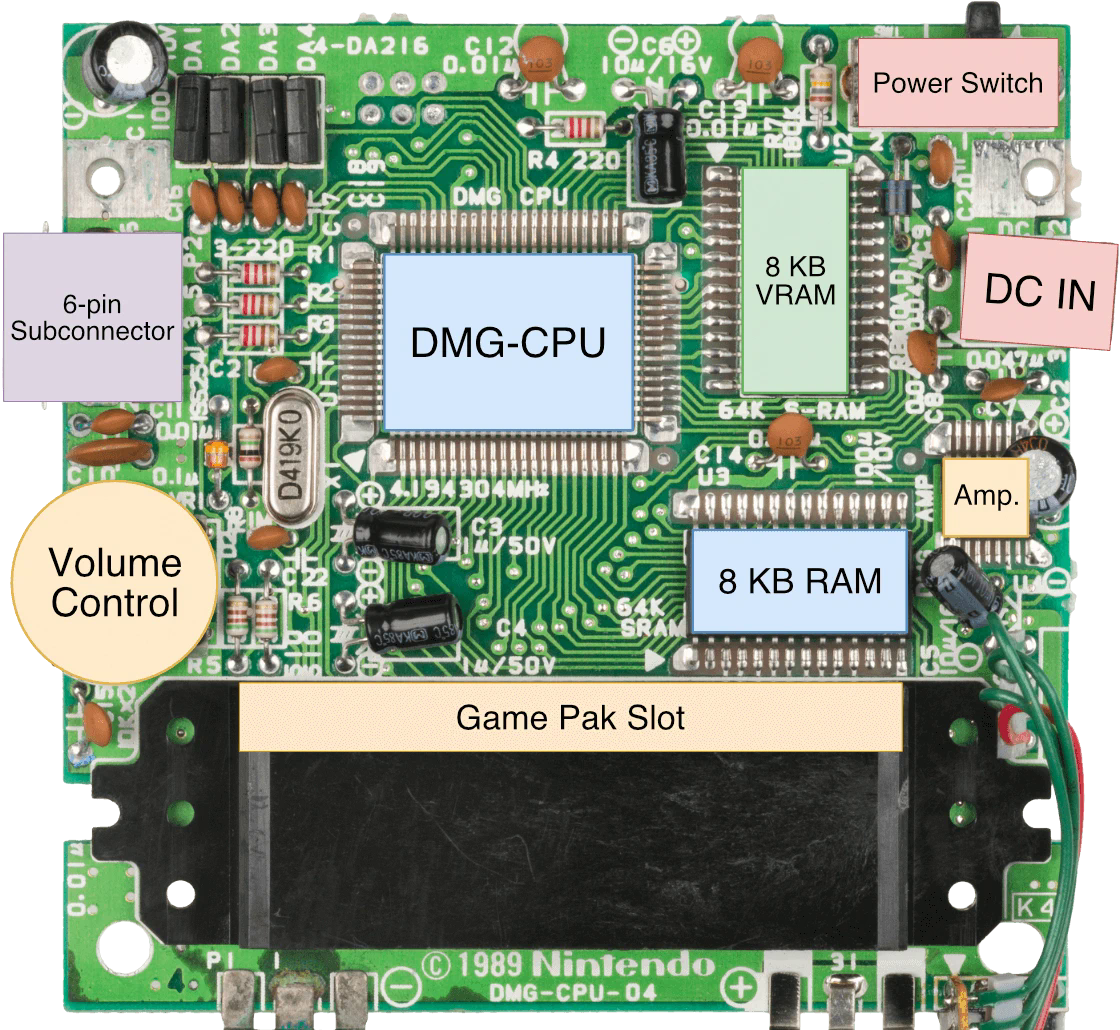
\includegraphics[width=0.9\linewidth]{dmg_marked.png}
		\caption{Zdjęcie płyty głównej oryginalnego Game Boy'a z opisami kompomentów\cite{copetti}}
		\label{fig:marked_dmg}
	\end{minipage}
	\hfill
	\begin{minipage}{0.45\textwidth}
		\centering
		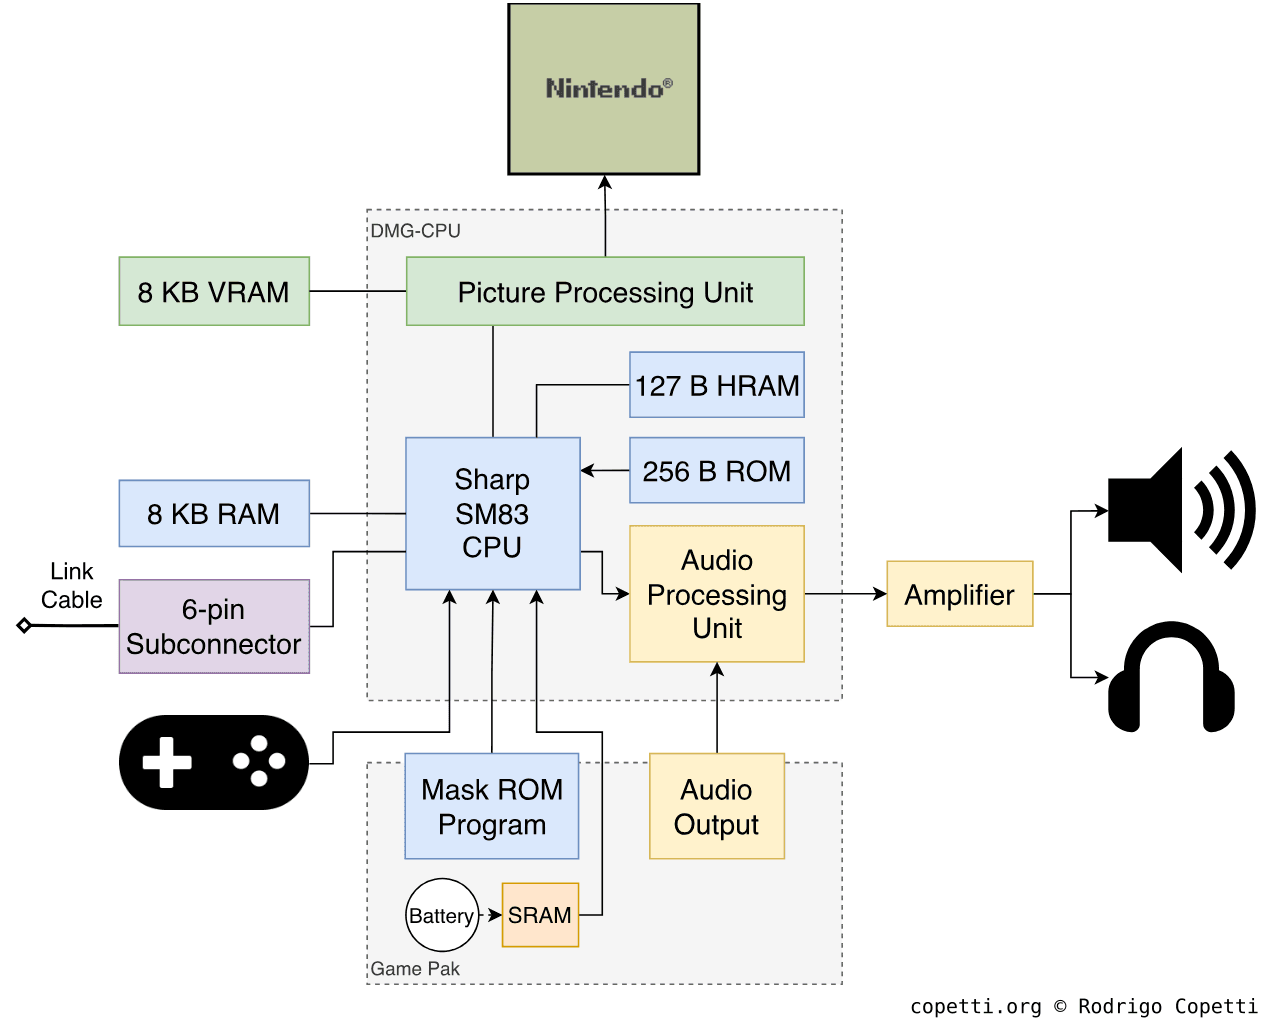
\includegraphics[width=0.9\linewidth]{dmg_chart.png}
		\caption{Schemat płyty głównej konsoli Game Boy\cite{copetti}}
		\label{fig:chart_dmg}
	\end{minipage}
\end{figure}

\subsubsection{Jednostka centralna}

Centralnym elementem płyty głównej jest układ DMG-CPU, stanowiący zintegrowany system typu System on Chip (SoC). W przeciwieństwie do klasycznych konstrukcji mikrokomputerowych, w których poszczególne funkcje realizowane są przez oddzielne układy scalone, DMG-CPU integruje w jednej strukturze półprzewodnikowej jednostkę obliczeniową, kontroler pamięci, układ graficzny, generator dźwięku oraz logikę sterującą systemem.

Rdzeń obliczeniowy układu bazuje na architekturze 8-bitowej z 16-bitową przestrzenią adresową i realizuje wykonywanie programu oraz zarządzanie przepływem danych pomiędzy komponentami systemu. Integracja funkcji w jednym układzie pozwoliła na ograniczenie liczby połączeń na płycie głównej, zmniejszenie poboru energii oraz zwiększenie niezawodności urządzenia.

DMG-CPU odpowiada również za synchronizację pracy podsystemów, obsługę przerwań sprzętowych, sterowanie dostępem do pamięci operacyjnej i wideo oraz koordynację komunikacji z interfejsem kartridża i urządzeniami wejścia-wyjścia. Zastosowanie architektury SoC stanowiło kluczowy element miniaturyzacji konsoli oraz umożliwiło osiągnięcie wysokiej efektywności energetycznej przy zachowaniu pełnej funkcjonalności systemu.


\subsubsection{Pamięć operacyjna i pamięć wideo}

Na płycie głównej znajdują się układy pamięci pełniące różne funkcje w architekturze systemu:

\begin{itemize}
	\item \textbf{WRAM (Work RAM)} -- pamięć operacyjna wykorzystywana przez procesor do przechowywania danych roboczych oraz stosu.
	\item \textbf{VRAM (Video RAM)} -- pamięć przeznaczona do przechowywania danych graficznych, takich jak mapy kafli, wzorce znaków oraz informacje o sprite’ach.
\end{itemize}

Pamięci te współpracują bezpośrednio z procesorem oraz układem generowania obrazu, zapewniając sprawną wymianę danych niezbędnych do działania systemu.

\subsubsection{Układ graficzny}

Funkcje generowania obrazu realizowane są przez zintegrowany kontroler LCD, który odpowiada za przetwarzanie danych graficznych i sterowanie wyświetlaczem ciekłokrystalicznym. Układ ten obsługuje system kafli (tile-based graphics), renderowanie sprite’ów oraz synchronizację obrazu z odświeżaniem ekranu. Kontroler LCD współpracuje bezpośrednio z pamięcią wideo oraz procesorem, tworząc kompletny tor przetwarzania grafiki.

\subsubsection{Układ dźwiękowy}

System dźwiękowy konsoli jest zintegrowany z architekturą płyty głównej i składa się z generatorów fal dźwiękowych sterowanych programowo. Układ ten umożliwia generowanie kilku kanałów audio, w tym fal prostokątnych, szumu oraz próbek o ograniczonej rozdzielczości. Sygnał audio kierowany jest następnie do wzmacniacza i głośnika lub wyjścia słuchawkowego. Ze względu skomplikowania, kompoment układu dźwiękowego nie będzie uwzględniany w implementacji.

\subsubsection{Interfejs kartridża}

Na płycie głównej znajduje się złącze kartridża umożliwiające komunikację z zewnętrznym nośnikiem oprogramowania. Interfejs ten zapewnia:

\begin{itemize}
	\item dostęp do pamięci programu,
	\item komunikację z dodatkowymi układami w kartridżu,
	\item możliwość rozszerzenia funkcjonalności systemu.
\end{itemize}

Zastosowanie wymiennych kartridży umożliwiło modularną architekturę systemu oraz łatwą dystrybucję oprogramowania.

\subsubsection{Układy wejścia i wyjścia}

Płyta główna integruje również komponenty odpowiedzialne za komunikację z użytkownikiem oraz otoczeniem:

\begin{itemize}
	\item kontroler przycisków sterujących,
	\item interfejs komunikacyjny (port szeregowy),
	\item sterowanie wyświetlaczem LCD,
	\item wzmacniacz audio.
\end{itemize}

Układy te zapewniają interakcję użytkownika z systemem oraz obsługę sygnałów wejściowych i wyjściowych.

Płyta główna konsoli Game Boy stanowi przykład zwartej i funkcjonalnej integracji elementów elektronicznych w systemie o ograniczonych zasobach sprzętowych. Zastosowanie zintegrowanych układów scalonych, zoptymalizowane zarządzanie energią oraz modułowa struktura pamięci i interfejsów umożliwiły stworzenie wydajnego, przenośnego systemu rozrywkowego. Analiza budowy płyty głównej pozwala dostrzec kompromis pomiędzy funkcjonalnością, energooszczędnością a prostotą konstrukcji, charakterystyczny dla projektowania urządzeń przenośnych końca XX wieku.

\subsection{Kartridże systemu Game Boy}

Kartridże stanowią podstawowy nośnik oprogramowania dla konsoli Game Boy oraz element rozszerzający funkcjonalność systemu. Oprócz pamięci programu zawierają one układy logiczne odpowiedzialne za zarządzanie pamięcią, zapisywanie danych użytkownika oraz, w niektórych przypadkach, dodatkowe funkcje sprzętowe. Różnorodność konstrukcji kartridżów wynikała z konieczności obsługi gier o rosnącej złożoności przy zachowaniu ograniczeń architektury systemu.

\subsubsection{Kartridże bez kontrolera banków pamięci (ROM Only)}

Najprostszy typ kartridża zawiera wyłącznie pamięć ROM z programem gry. Konstrukcja ta nie umożliwia przełączania banków pamięci ani zapisu danych użytkownika. Ze względu na ograniczoną pojemność stosowana była głównie w prostszych produkcjach we wczesnym okresie rozwoju systemu.

\subsubsection{Kartridże z kontrolerem MBC1}

Kontroler Memory Bank Controller 1 (MBC1) umożliwia przełączanie banków pamięci ROM oraz, opcjonalnie, banków pamięci RAM. Układ ten pozwalał na znaczące zwiększenie maksymalnego rozmiaru programu. Kartridże tego typu występowały w kilku wariantach:

\begin{itemize}
	\item MBC1 + RAM,
	\item MBC1 + RAM + bateria podtrzymująca zapis danych.
\end{itemize}

\subsubsection{Kartridże z kontrolerem MBC2}

MBC2 integruje funkcję przełączania banków ROM z niewielką, wbudowaną pamięcią RAM przeznaczoną do zapisu danych gry. W odróżnieniu od innych kontrolerów, pamięć RAM jest integralną częścią układu i nie występuje jako oddzielny komponent. Kartridże te standardowo wyposażone były w baterię podtrzymującą zapis.

\subsubsection{Kartridże z kontrolerem MBC3}

MBC3 rozszerza funkcjonalność poprzednich kontrolerów o zegar czasu rzeczywistego (RTC). Rozwiązanie to umożliwiało implementację mechanik zależnych od upływu czasu rzeczywistego. Warianty konstrukcyjne obejmowały:

\begin{itemize}
	\item MBC3 + RAM,
	\item MBC3 + RAM + bateria,
	\item MBC3 + RAM + bateria + RTC.
\end{itemize}
\subsubsection{Kartriże z kontrolerem MBC4}
W dokumentacji platformy spotykana jest również wzmianka o kontrolerze MBC4. Jednak dostępne źródła nie dostarczają jednoznacznych dowodów na jego wykorzystanie w komercyjnych kartridżach Game Boy. Z tego względu w wielu opracowaniach przyjmuje się, że układ ten nie został wykorzystany w praktyce lub jego zastosowanie było bardzo ograniczone.
\subsubsection{Kartridże z kontrolerem MBC5}

MBC5 wprowadza rozszerzony system adresowania pamięci ROM oraz obsługę większych pojemności pamięci RAM. Układ ten był stosowany w późniejszych produkcjach o dużej objętości danych. Warianty obejmowały:

\begin{itemize}
	\item MBC5 + RAM,
	\item MBC5 + RAM + bateria,
	\item MBC5 + RAM + bateria + silnik wibracyjny (Rumble).
\end{itemize}

\subsubsection{Kartridże specjalizowane}

Oprócz standardowych kontrolerów banków pamięci produkowano kartridże wyposażone w dodatkowe układy funkcjonalne rozszerzające możliwości systemu. Do najważniejszych należą:

\begin{itemize}
	\item kartridże z czujnikiem ruchu,
	\item kartridże z pamięcią EEPROM,
	\item kartridże z dodatkowymi układami logicznymi sterującymi akcesoriami,
	\item kartridże diagnostyczne i testowe wykorzystywane w procesie produkcyjnym.
\end{itemize}

\subsubsection{Struktura fizyczna kartridża}

Typowy kartridż składa się z płytki drukowanej zawierającej układ ROM, opcjonalną pamięć RAM, kontroler banków pamięci oraz element podtrzymania zasilania pamięci zapisu. Komunikacja z konsolą odbywa się za pośrednictwem złącza krawędziowego, które zapewnia dostęp do magistrali adresowej, magistrali danych oraz linii sterujących.
\newpage
\section{Model działania systemu Game Boy}
\subsection{Inicjalizacja systemu}

Proces inicjalizacji systemu rozpoczyna się bezpośrednio po podaniu zasilania i stanowi sekwencję operacji przygotowujących komponenty sprzętowe do poprawnego wykonywania programu użytkownika. Etap ten obejmuje ustawienie stanu początkowego procesora, konfigurację rejestrów sterujących, inicjalizację pamięci oraz przygotowanie układu graficznego do generowania obrazu.

\subsubsection{Stan początkowy procesora}

Po uruchomieniu systemu procesor rozpoczyna wykonywanie kodu spod zdefiniowanego adresu startowego. Rejestry procesora oraz wskaźniki systemowe przyjmują wartości początkowe określone przez logikę sprzętową. W tym etapie przygotowywany jest stos, a licznik programu kierowany jest do procedury inicjalizacyjnej.

W początkowej fazie globalny mechanizm obsługi przerwań pozostaje wyłączony, co zapobiega zakłóceniu procesu konfiguracji systemu przez zdarzenia asynchroniczne.

\subsubsection{Konfiguracja pamięci i przestrzeni adresowej}

Procedura inicjalizacji obejmuje przygotowanie obszarów pamięci wykorzystywanych przez system. Dane w pamięci operacyjnej mogą zostać wyzerowane lub ustawione na wartości domyślne, a rejestry sterujące urządzeń peryferyjnych otrzymują konfigurację początkową.

Istotnym elementem jest także przygotowanie struktur danych wykorzystywanych przez układ graficzny, w szczególności map tła oraz danych obiektów. W tym etapie możliwe jest również przygotowanie obszarów buforowych przeznaczonych do późniejszego wykorzystania przez program użytkownika.

\subsubsection{Inicjalizacja układu graficznego}

Układ graficzny zostaje skonfigurowany poprzez zapis odpowiednich wartości do rejestrów sterujących. Konfiguracja obejmuje włączenie wyświetlania obrazu, ustawienie parametrów renderowania tła oraz przygotowanie pamięci przechowującej dane graficzne.

W początkowej fazie generowanie obrazu może być czasowo wstrzymane, co umożliwia bezpieczne przygotowanie danych w pamięci wideo oraz pamięci atrybutów obiektów. Po zakończeniu konfiguracji układ graficzny przechodzi do trybu normalnej pracy i rozpoczyna cykliczne generowanie klatek obrazu.

\subsubsection{Przygotowanie systemu przerwań}

Po zakończeniu konfiguracji podstawowych komponentów system aktywuje wybrane źródła przerwań. Rejestr maskujący przerwania zostaje ustawiony zgodnie z wymaganiami programu, a następnie globalna obsługa przerwań może zostać włączona.

Aktywacja mechanizmu przerwań umożliwia synchronizację działania programu z układami peryferyjnymi oraz reagowanie na zdarzenia zachodzące w systemie w czasie rzeczywistym.

\subsubsection{Przekazanie sterowania programowi użytkownika}

Końcowym etapem inicjalizacji jest przekazanie sterowania właściwemu programowi wykonywalnemu. Od tego momentu system pracuje w trybie operacyjnym, a dalsze działanie konsoli jest determinowane przez kod programu oraz zdarzenia sprzętowe.

\subsubsection{Znaczenie procesu inicjalizacji}

Poprawna inicjalizacja systemu stanowi warunek konieczny stabilnego działania wszystkich komponentów sprzętowych. Sekwencja operacji wykonywanych po uruchomieniu zapewnia spójność konfiguracji urządzeń, deterministyczny stan początkowy systemu oraz przygotowanie środowiska wykonawczego dla programu użytkownika.
\subsection{Cykl pracy procesora}

Procesor zastosowany w konsoli Game Boy jest 8-bitową jednostką opartą na zmodyfikowanej architekturze zbliżonej do Z80. Jego działanie jest determinowane przez cykl zegara systemowego oraz mechanizm wykonywania instrukcji w modelu sekwencyjnym. Zrozumienie cyklu pracy procesora jest kluczowe dla analizy działania całego systemu, ponieważ CPU koordynuje komunikację pomiędzy pamięcią, układem graficznym oraz urządzeniami wejścia/wyjścia.

\subsubsection{Model cyklu rozkazowego}

Podstawowy cykl pracy procesora można opisać jako powtarzającą się sekwencję trzech etapów:
\begin{enumerate}
	\item pobranie instrukcji z pamięci,
	\item dekodowanie instrukcji,
	\item wykonanie instrukcji.
\end{enumerate}

W pierwszym etapie procesor odczytuje kod operacji spod adresu wskazywanego przez licznik programu (PC). Następnie licznik programu zostaje inkrementowany, a pobrana wartość trafia do wewnętrznego rejestru instrukcji.

W drugim etapie następuje interpretacja kodu operacji oraz ustalenie wymaganych operandów. Proces dekodowania determinuje, czy instrukcja wymaga dodatkowych danych z pamięci oraz jakie jednostki funkcjonalne procesora zostaną zaangażowane w jej wykonanie.

Trzeci etap obejmuje właściwe wykonanie operacji arytmetycznej, logicznej lub sterującej. W zależności od typu instrukcji może to obejmować operacje na rejestrach, dostęp do pamięci lub zmianę przepływu sterowania programu.

\subsubsection{Synchronizacja z zegarem systemowym}

Procesor pracuje synchronicznie z zegarem systemowym, którego częstotliwość determinuje tempo wykonywania operacji. Każda instrukcja wymaga określonej liczby cykli zegara do wykonania. Czas realizacji instrukcji nie jest stały i zależy od jej złożoności oraz liczby operacji pamięciowych.

Istotnym elementem synchronizacji jest współdzielenie magistrali danych z innymi komponentami systemu. Dostęp do pamięci jest realizowany w ściśle określonych momentach cyklu zegara, co zapewnia spójność transmisji danych pomiędzy CPU a pozostałymi układami.

\subsubsection{Dostęp do pamięci i operacje magistrali}

Procesor komunikuje się z pamięcią poprzez magistralę adresową i magistralę danych. W trakcie cyklu rozkazowego mogą wystąpić operacje odczytu lub zapisu pamięci. Operacje te są wykonywane sekwencyjnie i blokują dostęp do magistrali dla innych komponentów na czas trwania transferu.

Mapowanie pamięci odgrywa istotną rolę w cyklu pracy procesora, ponieważ różne zakresy adresowe odpowiadają różnym typom zasobów systemowych, takim jak pamięć operacyjna, pamięć wideo oraz rejestry sterujące urządzeń peryferyjnych.

\subsubsection{Obsługa przerwań}

Cykl pracy procesora może zostać przerwany przez mechanizm przerwań sprzętowych. Wystąpienie przerwania powoduje czasowe wstrzymanie wykonywania bieżącego programu oraz zapis aktualnego stanu procesora na stosie.

Po zaakceptowaniu przerwania procesor przechodzi do procedury obsługi przerwania wskazanej w tablicy wektorów przerwań. Po zakończeniu obsługi następuje przywrócenie poprzedniego stanu procesora i kontynuacja wykonywania programu od miejsca przerwania.

\subsubsection{Znaczenie cyklu pracy dla działania systemu}

Deterministyczny charakter cyklu pracy procesora umożliwia precyzyjną synchronizację z układem graficznym oraz pozostałymi komponentami systemu. W szczególności liczba cykli zegara zużywana przez instrukcje wpływa bezpośrednio na generowanie obrazu oraz obsługę zdarzeń wejścia/wyjścia.

Analiza cyklu pracy procesora stanowi podstawę do modelowania działania systemu oraz jest niezbędna przy implementacji oprogramowania emulującego działanie konsoli.
\subsection{Magistrala pamięciowa i charakterystyka działania pamięci}

System pamięci konsoli Game Boy opiera się na wspólnej przestrzeni adresowej obsługiwanej przez procesor oraz na zestawie wyspecjalizowanych obszarów pamięci o odmiennych funkcjach. Komunikacja pomiędzy jednostką centralną a zasobami pamięciowymi realizowana jest za pomocą magistrali adresowej, magistrali danych oraz sygnałów sterujących, które determinują kierunek i tryb transferu informacji.

\subsubsection{Organizacja magistrali pamięciowej}

Magistrala adresowa umożliwia wskazanie konkretnej komórki pamięci w przestrzeni adresowej systemu. Procesor generuje adres, który identyfikuje zasób, z którego ma nastąpić odczyt danych lub do którego ma zostać wykonany zapis. Magistrala danych służy do przesyłania właściwych informacji pomiędzy procesorem a wskazanym komponentem systemu.

Operacje pamięciowe są synchronizowane z zegarem systemowym. W każdym cyklu dostępu do pamięci następuje ustalenie adresu, aktywacja sygnału sterującego oraz transfer danych. Ze względu na współdzielenie magistrali przez różne komponenty systemu dostęp do niej jest ściśle kontrolowany, co zapobiega konfliktom transmisji.

\subsubsection{Mapowanie przestrzeni adresowej}

Przestrzeń adresowa systemu jest podzielona na logiczne segmenty odpowiadające różnym typom zasobów sprzętowych. Poszczególne zakresy adresów są przypisane do pamięci programu, pamięci operacyjnej, pamięci wideo oraz rejestrów sterujących urządzeń peryferyjnych.

Mapowanie pamięci pełni funkcję mechanizmu integrującego różnorodne komponenty sprzętowe w jednolitą przestrzeń adresową. Dzięki temu procesor może komunikować się z układami systemowymi za pomocą standardowych operacji odczytu i zapisu, bez konieczności stosowania odrębnych instrukcji wejścia/wyjścia.

\subsubsection{Rodzaje pamięci w systemie}

W architekturze systemu można wyróżnić kilka podstawowych typów pamięci:

\begin{itemize}
	\item pamięć programu (ROM), zawierająca kod wykonywalny oraz dane statyczne,
	\item pamięć operacyjna (RAM), wykorzystywana do przechowywania danych tymczasowych,
	\item pamięć wideo (VRAM), przeznaczona do przechowywania danych graficznych,
	\item rejestry urządzeń peryferyjnych odwzorowane w przestrzeni adresowej.
\end{itemize}

Każdy z wymienionych typów pamięci charakteryzuje się odmiennym przeznaczeniem funkcjonalnym oraz sposobem dostępu. W szczególności pamięć wideo jest współdzielona z układem graficznym, co wprowadza ograniczenia czasowe w dostępie do niej przez procesor.

\subsubsection{Charakterystyka operacji pamięciowych}

Operacje pamięciowe wykonywane przez procesor obejmują odczyt danych, zapis danych oraz transfery blokowe realizowane sekwencyjnie. Czas trwania operacji zależy od rodzaju pamięci oraz liczby cykli zegara wymaganych do realizacji transferu.

Dostęp do pamięci może być ograniczony przez stan systemu, w szczególności przez aktywność układów współdzielących magistralę. W określonych fazach pracy systemu wybrane obszary pamięci mogą być czasowo niedostępne dla procesora lub dostępne jedynie w określonych warunkach synchronizacji.

\subsubsection{Rola systemu pamięci w działaniu konsoli}

Architektura pamięci stanowi podstawę wymiany informacji pomiędzy wszystkimi komponentami systemu. Determinuje ona sposób wykonywania programu, obsługi grafiki oraz komunikacji z urządzeniami wejścia/wyjścia.

Jednolita przestrzeń adresowa oraz deterministyczny model dostępu do pamięci umożliwiają przewidywalne działanie systemu w czasie rzeczywistym. Właściwości te mają istotne znaczenie zarówno dla analizy architektury sprzętowej, jak i dla implementacji oprogramowania odwzorowującego działanie systemu.
\subsection{Generowanie klatki obrazu}

Generowanie obrazu w konsoli Game Boy jest realizowane przez układ graficzny (PPU), który współpracuje z pamięcią wideo oraz pamięcią atrybutów obiektów. Proces ten przebiega cyklicznie i jest ściśle zsynchronizowany z zegarem systemowym oraz działaniem procesora. Obraz powstaje poprzez sekwencyjne renderowanie tła, a następnie nakładanie obiektów ruchomych zapisanych w pamięci OAM (Rozdział \ref{oam}).

\subsubsection{Format zapisu grafiki w pamięci VRAM}

Podstawową jednostką reprezentacji obrazu w systemie jest tzw. kafel (ang. tile). Każdy kafel reprezentuje fragment obrazu o wymiarach 8×8 pikseli. Dane kafli przechowywane są w pamięci wideo (VRAM) w postaci uporządkowanej tablicy bajtów.

Każdy wiersz kafla kodowany jest przy użyciu dwóch bajtów, które reprezentują dwubitową informację o kolorze każdego piksela w wierszu. Pierwszy bajt zawiera najmniej znaczące bity wartości koloru, natomiast drugi bajt zawiera bity najbardziej znaczące. Odczyt odpowiadających sobie bitów z obu bajtów pozwala określić indeks koloru dla pojedynczego piksela.

Układ graficzny interpretuje dane kafli na podstawie mapy tła, która przechowuje indeksy kafli oraz ich rozmieszczenie na ekranie. Dzięki temu możliwe jest wielokrotne wykorzystanie tych samych danych graficznych w różnych miejscach obrazu.

\subsubsection{Renderowanie tła}

Proces generowania klatki rozpoczyna się od renderowania tła. Układ graficzny przetwarza mapę tła linia po linii, odczytując odpowiednie indeksy kafli oraz ich dane z pamięci VRAM. Dla każdej linii obrazu wyznaczany jest odpowiedni fragment kafla, który następnie przekształcany jest w wartości kolorów pikseli.

Renderowanie odbywa się w sposób deterministyczny i jest zsynchronizowane z aktualną pozycją skanowania ekranu. W wyniku tego procesu powstaje podstawowa warstwa obrazu, która stanowi bazę dla dalszego etapu renderowania.

\subsubsection{Pamięć OAM i reprezentacja obiektów}
\label{oam}
OAM (Object Attribute Memory) jest wyspecjalizowanym obszarem pamięci przeznaczonym do przechowywania informacji o obiektach ruchomych, określanych jako sprite'y. Pamięć ta zawiera zestaw rekordów opisujących właściwości graficzne oraz położenie obiektów wyświetlanych na ekranie.

Każdy wpis w pamięci OAM zawiera:
\begin{itemize}
	\item współrzędną pionową obiektu na ekranie,
	\item współrzędną poziomą obiektu,
	\item indeks kafla opisującego grafikę obiektu,
	\item zestaw atrybutów określających sposób renderowania.
\end{itemize}

Atrybuty obiektu mogą obejmować informacje o priorytecie wyświetlania, odbiciu lustrzanym oraz wyborze palety kolorów. Układ graficzny odczytuje zawartość pamięci OAM podczas procesu generowania obrazu i wykorzystuje ją do nałożenia obiektów na wcześniej wyrenderowane tło.

\subsubsection{Renderowanie obiektów}

Po wygenerowaniu warstwy tła układ graficzny przystępuje do renderowania obiektów zapisanych w pamięci OAM. Dla każdej linii obrazu wybierane są obiekty znajdujące się w jej obszarze, a następnie ich dane graficzne są pobierane z pamięci VRAM.

Renderowanie obiektów polega na nałożeniu ich pikseli na istniejący obraz tła zgodnie z regułami priorytetu. W przypadku kolizji pikseli o różnych źródłach decyzja o widoczności zależy od atrybutów obiektu oraz wartości koloru tła.

\subsubsection{DMA i bezpośredni transfer danych do OAM}

W celu usprawnienia transferu danych do pamięci OAM system wykorzystuje mechanizm DMA (Direct Memory Access). Mechanizm ten umożliwia bezpośrednie kopiowanie bloków danych z określonego obszaru pamięci do pamięci OAM bez konieczności wykonywania instrukcji kopiowania przez procesor.

Transfer DMA polega na automatycznym odczycie kolejnych bajtów ze źródłowego obszaru pamięci oraz ich zapisie do kolejnych komórek pamięci OAM. W trakcie operacji DMA procesor ma ograniczony dostęp do magistrali pamięci, co zapewnia spójność przesyłanych danych.

Zastosowanie mechanizmu bezpośredniego transferu bajtów umożliwia szybkie aktualizowanie danych obiektów, co jest szczególnie istotne w systemach czasu rzeczywistego, gdzie konieczna jest synchronizacja zmian graficznych z generowaniem kolejnych klatek obrazu.

\subsection{System przerwań}

Mechanizm przerwań w konsoli Game Boy umożliwia asynchroniczną reakcję procesora na zdarzenia sprzętowe zachodzące w systemie. Zamiast ciągłego odpytywania stanu urządzeń peryferyjnych, procesor może wykonywać program główny, a w momencie wystąpienia określonego zdarzenia przejść do dedykowanej procedury obsługi przerwania. Rozwiązanie to zwiększa efektywność wykorzystania czasu procesora oraz zapewnia deterministyczną obsługę zdarzeń czasowych.

\subsubsection{Warunki występowania przerwań}

Przerwanie może zostać wygenerowane przez układ sprzętowy po spełnieniu określonego warunku logicznego, takiego jak zakończenie operacji wejścia/wyjścia, osiągnięcie zadanego stanu licznika czasowego lub zmiana stanu kontrolera wejściowego. Aby przerwanie zostało obsłużone, muszą zostać spełnione trzy warunki:
\begin{enumerate}
	\item źródło przerwania zgłosi żądanie,
	\item odpowiedni typ przerwania jest odblokowany w rejestrze maskującym,
	\item globalny mechanizm obsługi przerwań w procesorze jest aktywny.
\end{enumerate}

Jeżeli wszystkie warunki są spełnione, procesor kończy wykonywanie bieżącej instrukcji, zapisuje aktualny stan wykonania programu oraz przechodzi do procedury obsługi przerwania.

\subsubsection{Rodzaje przerwań}



Każdy typ przerwania (tabela \ref{tab:gb_interrupts}) posiada przypisany wektor, czyli stały adres w pamięci programu, pod którym rozpoczyna się procedura jego obsługi. Priorytet przerwań jest ustalony sprzętowo i determinuje kolejność ich obsługi w przypadku jednoczesnego wystąpienia kilku zdarzeń.

\subsubsection{Przebieg obsługi przerwania}

Obsługa przerwania przebiega według ściśle określonej sekwencji działań wykonywanych przez procesor:
\begin{enumerate}
	\item zakończenie wykonywania bieżącej instrukcji,
	\item zapis aktualnej wartości licznika programu na stosie,
	\item czasowe zablokowanie dalszych przerwań,
	\item przejście do adresu procedury obsługi przerwania,
	\item wykonanie kodu obsługi zdarzenia,
	\item przywrócenie poprzedniego stanu programu i kontynuacja wykonania.
\end{enumerate}

Zapis stanu programu na stosie umożliwia powrót do przerwanego miejsca po zakończeniu obsługi. Instrukcja powrotu z przerwania przywraca licznik programu oraz ponownie aktywuje globalny mechanizm przerwań.

\subsubsection{Funkcje realizowane przez przerwania}

Przerwania pełnią w systemie rolę mechanizmu synchronizującego działanie procesora z procesami zachodzącymi w układach peryferyjnych. Do najważniejszych funkcji realizowanych za ich pomocą należą:
\begin{itemize}
	\item synchronizacja zmian graficznych z cyklem generowania obrazu,
	\item odmierzanie czasu oraz generowanie zdarzeń okresowych,
	\item obsługa transmisji danych pomiędzy komponentami systemu,
	\item reagowanie na działania użytkownika.
\end{itemize}

W szczególności przerwanie synchronizacji pionowej umożliwia bezpieczną aktualizację danych graficznych w pamięci wideo w momentach, gdy układ graficzny nie odczytuje danych do generowania obrazu. Mechanizm przerwań zapewnia tym samym spójność danych oraz stabilność działania systemu w czasie rzeczywistym.

\subsubsection{Znaczenie mechanizmu przerwań}

Zastosowanie przerwań pozwala na efektywne zarządzanie współbieżnymi zdarzeniami w systemie o ograniczonych zasobach sprzętowych. Deterministyczna obsługa zdarzeń oraz priorytetyzacja źródeł przerwań stanowią podstawę prawidłowego działania konsoli oraz umożliwiają implementację oprogramowania wymagającego precyzyjnej synchronizacji czasowej.

\newpage
\section{Implementacja}

\subsection{Wykorzystane narzędzia i zasoby}

Do implementacji emulatora zastosowano język C++\cite{stroustrup2022tour} ze względu na jego niskopoziomową naturę, wraz z bibliotekami Raylib  w wersji 5.0 \cite{raylib} dla implementancji graficznej i sterowania oraz  fmt w wersji 10.2.1 \cite{fmt} dla łatwiejszego formatowania tekstu.

\subsubsection{Funkcje biblioteki Raylib}

Funkcja \texttt{InitWindow()} inicjalizuje okno aplikacji oraz kontekst renderowania,
umożliwiając rozpoczęcie operacji graficznych. Cykl renderowania pojedynczej klatki
realizowany jest przy użyciu funkcji \texttt{BeginDrawing()} oraz \texttt{EndDrawing()},
pomiędzy którymi wykonywane są wszystkie operacje rysowania.

Do rysowania elementów graficznych wykorzystywane są następujące funkcje:
\begin{itemize}
	\item \texttt{ClearBackground()} -- czyści bufor renderowania i wypełnia go zadanym kolorem,
	\item \texttt{DrawText()} -- umożliwia prezentację tekstu,
	\item \texttt{DrawRectangle()} -- rysuje wypełniony prostokąt,
	\item \texttt{DrawLine()} -- rysuje linię,
	\item \texttt{DrawRectangleRec()} -- rysuje prostokąt na podstawie struktury \texttt{Rectangle},
	\item \texttt{DrawRectangleLines()} -- rysuje obrys prostokąta,
	\item \texttt{DrawRectangleLinesEx()} -- rysuje obrys prostokąta z kontrolą grubości linii.
\end{itemize}

Renderowanie tekstur realizowane jest przy użyciu:
\begin{itemize}
	\item \texttt{DrawTexture()} -- rysuje teksturę w zadanej pozycji,
	\item \texttt{DrawTextureEx()} -- rysuje teksturę z dodatkowymi transformacjami geometrycznymi,
	takimi jak skalowanie i obrót,
	\item \texttt{UpdateTexture()} -- aktualizuje zawartość tekstury w pamięci karty graficznej.
\end{itemize}

Operacje na danych obrazu w pamięci operacyjnej realizowane są przez:
\begin{itemize}
	\item \texttt{ImageClearBackground()} -- wypełnia obraz zadanym kolorem,
	\item \texttt{ImageDrawPixel()} -- umożliwia bezpośrednią modyfikację pojedynczych pikseli
	przed przesłaniem ich do tekstury.
\end{itemize}

Obsługa wejścia użytkownika realizowana jest przez:
\begin{itemize}
	\item \texttt{IsMouseButtonPressed()} -- wykrywa naciśnięcie przycisku myszy w bieżącej klatce,
	\item \texttt{IsKeyPressed()} -- wykrywa naciśnięcie klawisza klawiatury w bieżącej klatce.
\end{itemize}

Konfigurację działania biblioteki umożliwiają:
\begin{itemize}
	\item \texttt{SetTargetFPS()} -- ustala docelową częstotliwość generowania klatek,
	\item \texttt{SetTraceLogLevel()} -- konfiguruje poziom szczegółowości komunikatów diagnostycznych.
\end{itemize}

\subsubsection{Struktury biblioteki Raylib}

Biblioteka Raylib definiuje następujące struktury danych:
\begin{itemize}
	\item \texttt{Color} -- reprezentuje kolor w przestrzeni RGBA, zawiera składowe
	intensywności poszczególnych barw oraz przezroczystości,
	\item \texttt{Image} -- przechowuje dane obrazu w pamięci operacyjnej, w tym rozdzielczość,
	format pikseli oraz bufor danych graficznych,
	\item \texttt{Texture} -- reprezentuje teksturę przechowywaną w pamięci karty graficznej,
	wykorzystywaną w procesie renderowania.
\end{itemize}

\subsubsection{Funkcje biblioteki fmt}

Biblioteka \texttt{fmt} dostarcza następujące funkcje formatowania tekstu:
\begin{itemize}
	\item \texttt{fmt::print()} -- wyświetla sformatowany tekst na standardowym wyjściu,
	\item \texttt{fmt::println()} -- wyświetla sformatowany tekst zakończony znakiem nowej linii,
	\item \texttt{fmt::format()} -- zwraca sformatowany ciąg znaków bez jego wyświetlania,
	umożliwiając dalsze przetwarzanie tekstu w programie.
\end{itemize}


\subsection{Implementacja modułu obsługi kartridża}

Moduł kartridża odpowiada za wczytanie obrazu ROM z pliku binarnego, interpretację jego nagłówka oraz udostępnienie danych pamięci programu pozostałym komponentom emulatora. Implementacja została wykonana w języku C++ z wykorzystaniem standardowej biblioteki wejścia--wyjścia.

Stan kartridża przechowywany jest w strukturze \texttt{cart\_context}, która zawiera rozmiar pamięci ROM, wskaźnik na dane ROM, wskaźnik na strukturę nagłówka oraz nazwę pliku źródłowego. Dane ROM są ładowane do dynamicznie alokowanego bufora pamięci, natomiast nagłówek interpretowany jest poprzez rzutowanie fragmentu bufora na strukturę \texttt{rom\_header}. Zgodnie ze specyfikacją formatu ROM, nagłówek znajduje się pod adresem \texttt{0x100}.

\subsubsection{Struktura nagłówka ROM}

Informacje identyfikacyjne oraz parametry konfiguracyjne kartridża przechowywane są w nagłówku ROM. W implementacji nagłówek odwzorowano bezpośrednio jako strukturę języka C++, której układ odpowiada rozmieszczeniu danych w obrazie pamięci kartridża.

Struktura \texttt{rom\_header} zawiera następujące pola:

\begin{lstlisting}[style=cpp, label={lst:rom_header}, caption={Struktura \texttt{rom\_header}}]
	struct rom_header {
		uint8_t  entry[4];            // kod startowy
		uint8_t  nintendo_logo[0x30]; // dane graficzne logo producenta
		char     title[16];           // nazwa programu
		uint8_t  license_code;        // kod producenta
		uint8_t  new_license_code;    // rozszerzony kod producenta
		uint8_t  sgb_flag;            // flaga zgodnosci ze sprzetem
		uint8_t  type;                // typ kartridza i kontroler pamieci
		uint8_t  rom_size;            // rozmiar pamieci ROM
		uint8_t  ram_size;            // rozmiar pamieci RAM kartridza
		uint8_t  dest_code;           // kod regionu dystrybucji
		uint8_t  version;             // wersja programu
		uint8_t  checksum;            // suma kontrolna naglowka
		uint16_t global_checksum;     // suma kontrolna calego obrazu ROM
	};
\end{lstlisting}

Nagłówek znajduje się w pamięci ROM pod stałym adresem \texttt{0x100}. W implementacji dostęp do niego realizowany jest poprzez rzutowanie odpowiedniego fragmentu bufora pamięci na strukturę \texttt{rom\_header}. Takie podejście umożliwia bezpośredni odczyt pól nagłówka bez konieczności ręcznej interpretacji poszczególnych bajtów.

\paragraph{Interfejs dostępu}

Moduł kartridża udostępnia funkcję \texttt{get\_rom\_header()}, która zwraca wskaźnik na strukturę nagłówka. Pozwala to pozostałym komponentom emulatora na odczyt parametrów kartridża bez konieczności bezpośredniego dostępu do bufora pamięci ROM.

\subsubsection{Proces ładowania obrazu ROM}

Funkcja \texttt{cart\_load()} realizuje proces inicjalizacji kartridża. W pierwszym etapie plik otwierany jest w trybie binarnym, a następnie jego zawartość wczytywana jest w całości do pamięci operacyjnej. Po załadowaniu danych wyznaczany jest wskaźnik na strukturę nagłówka, z której odczytywane są podstawowe informacje identyfikacyjne.

W trakcie inicjalizacji prezentowane są następujące parametry kartridża:
\begin{itemize}
	\item tytuł programu,
	\item typ kartridża,
	\item rozmiar pamięci ROM,
	\item rozmiar pamięci RAM,
	\item kod licencyjny producenta,
	\item wersja ROM.
\end{itemize}

Interpretacja typu kartridża oraz kodu licencyjnego realizowana jest przy użyciu statycznych map odwzorowujących identyfikatory numeryczne na ich reprezentacje tekstowe.

\subsubsection{Dostęp do danych kartridża}

Moduł udostępnia interfejs umożliwiający dostęp do danych pamięci ROM przez pozostałe komponenty emulatora. Funkcja \texttt{cart\_read(uint16\_t address)} zwraca wartość bajtu znajdującego się pod wskazanym adresem pamięci kartridża. Dodatkowo moduł udostępnia funkcję \texttt{get\_rom\_header()}, umożliwiającą odczyt informacji nagłówkowych przez inne podsystemy emulatora.

Aktualna implementacja obsługuje wyłącznie kartridże typu \texttt{ROM ONLY}, bez mechanizmu bankowania pamięci.

\subsubsection{Weryfikacja poprawności nagłówka}

Poprawność nagłówka weryfikowana jest poprzez obliczenie sumy kontrolnej na podstawie danych znajdujących się w zakresie adresów \texttt{0x0134--0x014C}. Obliczona wartość porównywana jest z sumą kontrolną zapisaną w nagłówku ROM. Wynik weryfikacji prezentowany jest w postaci komunikatu diagnostycznego podczas inicjalizacji kartridża.

\subsubsection{Ograniczenia implementacji}

Obecna wersja modułu stanowi uproszczoną implementację mechanizmu obsługi kartridża. Nie zaimplementowano mechanizmów bankowania pamięci ani obsługi dodatkowych kontrolerów pamięci (MBC). Przyjęte podejście umożliwia jednak poprawne działanie programów wykorzystujących podstawowy model pamięci ROM.

\subsection{Implementacja magistrali systemowej}

Magistrala systemowa stanowi warstwę pośrednią pomiędzy procesorem a komponentami sprzętowymi emulatora. Jej zadaniem jest odwzorowanie przestrzeni adresowej systemu oraz przekierowanie operacji odczytu i zapisu do właściwych modułów funkcjonalnych. Implementacja magistrali realizuje zatem logiczne mapowanie adresów pamięci na odpowiadające im urządzenia peryferyjne lub obszary pamięci.

\subsubsection{Operacje odczytu z magistrali}

Podstawową funkcją magistrali jest procedura \texttt{bus\_read(uint16\_t address)}, która realizuje odczyt pojedynczego bajtu z przestrzeni adresowej. Funkcja analizuje wartość adresu i na tej podstawie deleguje operację do odpowiedniego komponentu emulatora.

Mapowanie przestrzeni adresowej jest opisana wcześniej w rozdziale 3.4

W przypadku trwającego transferu DMA dostęp do pamięci OAM jest blokowany, a magistrala zwraca wartość neutralną. Takie zachowanie odwzorowuje ograniczenia sprzętowe rzeczywistego systemu.

\subsubsection{Operacje zapisu do magistrali}

Procedura \texttt{bus\_write(uint16\_t address, uint8\_t value)} realizuje zapis danych do przestrzeni adresowej. Mechanizm działania jest analogiczny do operacji odczytu — adres determinuje komponent docelowy operacji zapisu.

Zapis do pamięci ROM przekazywany jest do kontrolera kartridża, co umożliwia obsługę mechanizmów bankowania pamięci. Operacje zapisu do pamięci wideo oraz pamięci roboczej przekierowywane są do odpowiednich modułów pamięciowych. W obszarach zarezerwowanych lub nieużywanych operacja zapisu jest ignorowana.

Szczególnym przypadkiem jest zapis do adresu \texttt{0xFFFF}, który modyfikuje rejestr maski przerwań procesora. Mechanizm ten pozwala na dynamiczne sterowanie systemem przerwań w trakcie działania programu.

\subsubsection{Operacje na słowach 16-bitowych}

Magistrala udostępnia również funkcje operujące na danych 16-bitowych:
\begin{itemize}
	\item \texttt{bus\_read16(address)} — odczyt dwóch kolejnych bajtów i ich złożenie w słowo 16-bitowe,
	\item \texttt{bus\_write16(address, value)} — zapis wartości 16-bitowej w postaci dwóch bajtów.
\end{itemize}

Operacje te wykorzystują konwencję zapisu w porządku little-endian, w której młodszy bajt przechowywany jest pod niższym adresem pamięci.

\subsubsection{Znaczenie architektoniczne magistrali}el


Zastosowanie scentralizowanej warstwy magistrali zapewnia:
\begin{itemize}
	\item jednoznaczne odwzorowanie przestrzeni adresowej systemu,
	\item izolację procesora od szczegółów implementacyjnych urządzeń peryferyjnych,
	\item możliwość łatwej rozbudowy emulatora o nowe komponenty,
	\item spójne modelowanie ograniczeń sprzętowych.
\end{itemize}

Magistrala stanowi zatem kluczowy element architektury emulatora, integrujący wszystkie moduły systemu w jednolitą strukturę komunikacyjną oraz zapewniający deterministyczne odwzorowanie zachowania sprzętu.
\subsection{Implementacja pamięci operacyjnej RAM}

Pamięć operacyjna systemu została odwzorowana w postaci struktury kontekstu zawierającej dwa fizycznie odrębne obszary pamięci: roboczą pamięć wewnętrzną WRAM oraz szybką pamięć wysoką HRAM. Oba segmenty reprezentowane są jako statyczne tablice bajtowe o stałym rozmiarze, co zapewnia deterministyczne odwzorowanie przestrzeni adresowej systemu.

Pamięć WRAM obejmuje zakres adresów od \texttt{0xC000} do \texttt{0xDFFF} i posiada rozmiar 8\,KB. Z kolei HRAM zajmuje obszar od \texttt{0xFF80} do \texttt{0xFFFF} z efektywnym rozmiarem 128\,B. Funkcja inicjalizacyjna ustawia wszystkie komórki obu obszarów na wartość początkową \texttt{0xFF}, co odpowiada stanowi pamięci po resecie systemu.

Dostęp do pamięci realizowany jest przez wyspecjalizowane funkcje odczytu i zapisu. Każda funkcja wykonuje translację adresu logicznego magistrali na indeks wewnętrznej tablicy poprzez odjęcie adresu bazowego segmentu (\textit{Listing \ref{lst:ram})}. W celu zapewnienia poprawności działania systemu implementacja zawiera kontrolę zakresu adresów. Próba dostępu poza dozwolony obszar skutkuje zgłoszeniem błędu i przerwaniem działania emulatora. Mechanizm ten zabezpiecza integralność modelu pamięci oraz ułatwia diagnostykę nieprawidłowych operacji.

\begin{lstlisting}[style=cpp,caption={Fragment implementacji pamięci operacyjnej},label={lst:ram}]

struct ram_context {
	std::array<uint8_t, 0x2000> wram;
	std::array<uint8_t, 0x80> hram;
};

static ram_context ctx;

uint8_t wram_read(uint16_t address) {
	auto err = fmt::format("ERROR: Invalid wram read address 0x{:X}", address); // Wiadomosc o blednym adresie
	address -= 0xC000; // Odjecie adresu bazowego segmentu dla wram, dajac nam indeks tablicy ctx.wram
	if (address >= 0x2000) { // Jesli  indeks wychodzi poza zakres tablicy, dajemy komunikat o bledzie i konczymy prace programu
		fmt::println(err);
		exit(-1);
	}
	return ctx.wram.at(address);
}
\end{lstlisting}


\subsection{Implementacja stosu procesora}

Stos procesora został zaimplementowany jako struktura danych działająca w przestrzeni pamięci systemowej i zarządzana przez rejestr wskaźnika stosu SP. Operacje na stosie wykorzystują interfejs magistrali systemowej, co zapewnia pełną zgodność z architekturą pamięci emulatora.

Operacja zapisu na stos realizowana jest poprzez dekrementację wskaźnika stosu, a następnie zapis wartości pod nowym adresem. Takie podejście odwzorowuje rzeczywiste działanie sprzętowego stosu, który rośnie w kierunku malejących adresów pamięci. Dla danych 16-bitowych stosowane są dwie kolejne operacje zapisu, rozpoczynające się od bajtu starszego, co zapewnia zgodność z reprezentacją little-endian.

Operacja odczytu ze stosu przebiega w odwrotnej kolejności. Najpierw odczytywana jest wartość spod adresu wskazywanego przez rejestr SP, a następnie wskaźnik stosu jest inkrementowany. W przypadku wartości 16-bitowych odczytywane są dwa kolejne bajty, które następnie łączone są w jedną wartość słowa maszynowego.

Takie podejście zapewnia pełną zgodność mechanizmu stosu z wymaganiami architektury procesora oraz umożliwia poprawną realizację instrukcji wywołań podprogramów, powrotów oraz obsługi przerwań.

\subsection{Implementacja systemowego licznika czasowego}

Odczyt instrukcji z tabeli opcodów w kontekście implementacji systemowego licznika czasowego powinien być zorganizowany w sposób przejrzysty i jednoznaczny. Każda instrukcja pobrana z tabeli opcodów odpowiada określonej liczbie cykli zegarowych, które bezpośrednio wpływają na aktualizację rejestru DIV. Po wykonaniu instrukcji emulator inkrementuje licznik DIV o liczbę cykli przypisaną do danej operacji.

Następnie, w oparciu o konfigurację rejestru TAC, analizowane są odpowiednie bity rejestru DIV w celu wykrycia opadającego zbocza sygnału zegarowego. W przypadku spełnienia warunku oraz aktywności licznika, następuje inkrementacja rejestru TIMA. Takie podejście zapewnia ścisłe powiązanie pomiędzy wykonywaniem instrukcji a mechanizmem odmierzania czasu.

Zaproponowany sposób integracji tabeli opcodów z systemem liczników czasowych umożliwia deterministyczne odwzorowanie zależności czasowych, gwarantując zgodność implementacji z semantyką sprzętową oraz poprawność działania emulatora.
\subsection{Implementacja procesora}

\subsubsection{Reprezentacja i przechowywanie instrukcji}

Najprostszym sposobem implementacji zestawu rozkazów procesora jest podejście naiwne, polegające na bezpośrednim powiązaniu każdego kodu operacji (\textit{opcode}) z jego implementacją przy użyciu rozbudowanej instrukcji warunkowej lub konstrukcji \texttt{switch-case}.

Choć metoda ta jest koncepcyjnie prosta, prowadzi do istotnych problemów projektowych:
\begin{itemize}
	\item silnego powiązania opisu instrukcji z jej implementacją,
	\item duplikacji logiki,
	\item ograniczonej skalowalności,
	\item utrudnionej rozbudowy i utrzymania kodu.
\end{itemize}

W celu eliminacji powyższych problemów zastosowano podejście rozdzielające:
\begin{enumerate}
	\item opis semantyki instrukcji,
	\item mechanizm dekodowania,
	\item mechanizm wykonania.
\end{enumerate}

Każda instrukcja reprezentowana jest przez strukturę danych zawierającą:
\begin{itemize}
	\item typ operacji,
	\item tryb adresowania,
	\item rejestry źródłowe i docelowe,
	\item warunek wykonania,
	\item parametr dodatkowy.
\end{itemize}

\begin{lstlisting}[style=cpp, caption={Struktura instrukcji}]
	struct instruction {
		in_type type{IN_NONE}; // Typ operacji
		addr_mode mode{AM_IMP}; // Tryb adresowania
		reg_type reg1{RT_NONE}; // Rejestry zrodlowy
		reg_type reg2{RT_NONE}; // Rejestr docelowy
		cond_type cond{CT_NONE}; // warunek wykonania
		uint8_t param{0}; // Parametr dodatkowy
	};
\end{lstlisting}



Struktury te przechowywane są w tablicy indeksowanej bezpośrednio kodem operacji. Proces dekodowania sprowadza się do odczytu odpowiedniej struktury na podstawie wartości \texttt{opcode}, natomiast wykonanie delegowane jest do wyspecjalizowanej procedury przypisanej do typu instrukcji.

Takie rozwiązanie zapewnia wyraźną separację odpowiedzialności, upraszcza rozszerzanie zestawu rozkazów oraz ułatwia implementację mechanizmów debugowania i trybów adresowania.


\begin{lstlisting}[style=cpp, caption={Fragment tablicy instrukcji indeksowanej kodem operacji}]
constexpr instruction instructions[0x100] = {
	// 0x0X
	
	[0x00] = {.type = IN_NOP, .mode = AM_IMP},
	[0x01] = {.type = IN_LD, .mode = AM_R_D16, .reg1 = RT_BC},
	[0x02] = {.type = IN_LD, .mode = AM_MR_R, .reg1 = RT_BC, .reg2 = RT_A},
	[0x03] = {.type = IN_INC, .mode = AM_R, .reg1 = RT_BC},
	[0x04] = {.type = IN_INC, .mode = AM_R, .reg1 = RT_B},
	[0x05] = {.type = IN_DEC, .mode = AM_R, .reg1 = RT_B},
	[0x06] = {.type = IN_LD, .mode = AM_R_D8, .reg1=RT_B},
	
	// Pozostale instrukcje...
}
\end{lstlisting}

\subsubsection{Struktura procesora i organizacja cyklu wykonawczego}

Implementacja CPU opiera się na centralnej strukturze kontekstu wykonania, przechowującej pełny stan procesora oraz dane pomocnicze wykorzystywane podczas dekodowania i realizacji instrukcji.


\begin{lstlisting}[style=cpp,caption={Kontekst wykonania procesora}]
	struct cpu_registers {
    	uint8_t A;
		uint8_t F;
		uint8_t B;
		uint8_t C;
		uint8_t D;
		uint8_t E;
		uint8_t H;
		uint8_t L;
		uint16_t PC;
		uint16_t SP;
	};
\end{lstlisting}


Stan architektoniczny przechowywany jest w strukturze \texttt{cpu\_registers}, zawierającej:

\textbf{Rejestry 8-bitowe:}
\begin{itemize}
	\item \texttt{A, F, B, C, D, E, H, L}
\end{itemize}

\textbf{Rejestry sterujące:}
\begin{itemize}
	\item \texttt{PC} --- licznik rozkazów (Program Counter),
	\item \texttt{SP} --- wskaźnik stosu (Stack Pointer).
\end{itemize}

Rejestr \texttt{F} pełni funkcję rejestru flag i zawiera bity statusowe:
\begin{itemize}
	\item Z --- flaga zera,
	\item N --- flaga odejmowania,
	\item H --- flaga półprzeniesienia,
	\item C --- flaga przeniesienia.
\end{itemize}

\begin{lstlisting}[style=cpp,caption={Kontekst wykonania procesora}]
	struct cpu_context {
		cpu_registers regs;
		uint32_t ticks; // Liczniki taktow procesora
		
		uint16_t fetch_data; // Pobrany operand
		uint16_t mem_destination; // adres docelowy zapisu
		bool dest_is_mem; // flaga zapisu do pamirci
		uint8_t op_code; // aktualny kod operacji
		instruction const* cur_instruction;  //wskaznik na strukture instrukcji
		
		
		bool int_master_enabled; // Globalne zezwolenie na przerwanie
		bool enabling_ime; // Flaga aktywacji przerwan
		bool halted; // 
		bool paused; // Stan zatrzymania procesora
		bool running; //
		
		uint8_t int_flags;
		uint8_t ie_register; // rejestr zgloszen
	};
\end{lstlisting}
Pełny stan wykonawczy przechowywany jest w strukturze \texttt{cpu\_context}, która oprócz rejestrów zawiera:



\textbf{Dane operacyjne:}
\begin{itemize}
	\item \texttt{ticks} --- licznik taktów procesora,
	\item \texttt{fetch\_data} --- pobrany operand,
	\item \texttt{mem\_destination} --- adres docelowy zapisu,
	\item \texttt{dest\_is\_mem} --- flaga zapisu do pamięci,
	\item \texttt{op\_code} --- aktualny kod operacji,
	\item \texttt{cur\_instruction} --- wskaźnik na strukturę instrukcji.
\end{itemize}

\textbf{Pola sterujące:}
\begin{itemize}
	\item globalne zezwolenie na przerwania,
	\item opóźnioną aktywację przerwań,
	\item stan zatrzymania procesora,
	\item rejestry zgłoszeń i masek przerwań.
\end{itemize}

\subsubsection{Organizacja cyklu wykonawczego}

\paragraph{Inicjalizacja}

Funkcja \texttt{cpu\_init()} ustawia stan początkowy procesora: inicjalizuje rejestry, ustawia wartości \texttt{PC} i \texttt{SP}, konfiguruje system przerwań oraz inicjalizuje pamięć emulatora.

\paragraph{Pobieranie i dekodowanie instrukcji}

Funkcja \texttt{fetch\_instruction()}:
\begin{enumerate}
	\item odczytuje kod operacji z pamięci pod adresem wskazywanym przez \texttt{PC},
	\item inkrementuje licznik rozkazów,
	\item wyszukuje strukturę opisującą instrukcję.
\end{enumerate}

\paragraph{Pobieranie operandów}

Funkcja \texttt{fetch\_data()} interpretuje tryb adresowania i przygotowuje dane dla etapu wykonania. Operandy mogą pochodzić z:
\begin{itemize}
	\item rejestrów procesora,
	\item pamięci operacyjnej,
	\item danych natychmiastowych zapisanych w kodzie programu.
\end{itemize}

Obsługiwane są także tryby autoinkrementacji i autodekrementacji.

\paragraph{Wykonanie instrukcji}

Funkcja \texttt{execute()} wybiera procedurę wykonawczą na podstawie typu operacji i przekazuje do niej kontekst procesora. Wykorzystanie tablicy wskaźników funkcji umożliwia szybkie mapowanie typu instrukcji na jej implementację.

\paragraph{Klasy procedur wykonawczych}

\textbf{Operacje arytmetyczne i logiczne:}
\begin{itemize}
	\item dodawanie, odejmowanie,
	\item operacje bitowe,
	\item porównania,
	\item aktualizacja flag statusowych.
\end{itemize}

\textbf{Operacje przepływu sterowania:}
\begin{itemize}
	\item skoki warunkowe i bezwarunkowe,
	\item wywołania i powroty,
	\item operacje na stosie.
\end{itemize}

\textbf{Instrukcje bitowe i rotacyjne:}
\begin{itemize}
	\item manipulacja pojedynczymi bitami,
	\item przesunięcia,
	\item rotacje.
\end{itemize}

\textbf{Instrukcje systemowe:}
\begin{itemize}
	\item zarządzanie przerwaniami,
	\item zatrzymanie procesora,
	\item operacje specjalne.
\end{itemize}

\paragraph{Symulacja cykli zegarowych}

Funkcja \texttt{emu\_cycles()} odpowiada za synchronizację systemu. Każdy cykl powoduje:
\begin{itemize}
	\item inkrementację \texttt{ticks},
	\item aktualizację timera,
	\item aktualizację układu graficznego,
	\item obsługę kontrolera DMA.
\end{itemize}

\paragraph{Główny krok procesora}

Funkcja \texttt{cpu\_step()} realizuje pojedynczy krok pracy CPU:
\begin{enumerate}
	\item pobranie instrukcji,
	\item symulację cyklu zegarowego,
	\item pobranie operandów,
	\item wykonanie instrukcji,
	\item obsługę przerwań,
	\item aktualizację transferów DMA.
\end{enumerate}

W stanie zatrzymania wykonywane są wyłącznie cykle zegarowe do momentu zgłoszenia przerwania.

\subsubsection{Warstwa dostępu do rejestrów}

Wprowadzono ujednoliconą warstwę dostępu do rejestrów 8- i 16-bitowych.

\paragraph{Odczyt rejestrów}

Funkcja \texttt{cpu\_read\_reg(reg\_type rt)}:
\begin{itemize}
	\item dla rejestrów 8-bitowych wykonuje bezpośredni odczyt,
	\item dla rejestrów złożonych (AF, BC, DE, HL) interpretuje pary rejestrów jako wartości 16-bitowe.
\end{itemize}

\paragraph{Zapis rejestrów}

Funkcja \texttt{cpu\_set\_reg(reg\_type rt, uint16\_t value)} umożliwia zapis wartości do wskazanego rejestru z zachowaniem spójności reprezentacji.

Dodatkowe funkcje \texttt{cpu\_read\_reg8} oraz \texttt{cpu\_set\_reg8} zapewniają bezpośredni dostęp do rejestrów bajtowych.

\paragraph{Zarządzanie flagami}

Funkcja \texttt{cpu\_set\_flags} umożliwia selektywną modyfikację flag statusowych oraz maskowanie niedozwolonych bitów rejestru \texttt{F}.

\subsubsection{Wykonanie w środowisku wielowątkowym}

Funkcja \texttt{cpu\_run\_threaded()} realizuje pracę procesora w dedykowanym wątku. Odpowiada za:
\begin{itemize}
	\item inicjalizację komponentów,
	\item ciągłe wykonywanie \texttt{cpu\_step()},
	\item zbieranie statystyk wydajności,
	\item synchronizację z modułem graficznym.
\end{itemize}

Oddzielenie cyklu CPU do dedykowanego wątku pozwala zachować stabilną prędkość emulacji oraz umożliwia równoległą obsługę warstwy prezentacji i interfejsu użytkownika.
\subsection{Implementacja przetwarzania grafiki}

Moduł przetwarzania grafiki odpowiada za emulację działania kontrolera LCD konsoli Game Boy. Jego zadaniem jest odwzorowanie rejestrów sterujących układu graficznego, zarządzanie paletami kolorów oraz obsługa komunikacji z magistralą pamięci emulatora. Implementacja została zaprojektowana w sposób modularny, tak aby możliwe było jednoznaczne odwzorowanie stanu sprzętowego w strukturze kontekstu oraz zapewnienie spójnego interfejsu dostępu do rejestrów.

\subsubsection{Reprezentacja rejestrów LCD i obsługa palet}

Stan kontrolera LCD przechowywany jest w strukturze \texttt{lcd\_context}. Struktura ta stanowi programowe odwzorowanie zestawu rejestrów sprzętowych oraz danych pomocniczych wykorzystywanych podczas procesu renderowania obrazu. W szczególności zawiera ona:

\begin{itemize}
	\item rejestry kontrolne \texttt{lcdc} oraz \texttt{lcds},
	\item rejestry przewijania obrazu \texttt{scroll\_x} oraz \texttt{scroll\_y},
	\item licznik aktualnie renderowanej linii \texttt{ly} oraz rejestr porównania \texttt{ly\_compare},
	\item rejestr odpowiedzialny za transfer DMA,
	\item rejestry palet kolorów dla tła oraz sprite'ów,
	\item współrzędne okna renderowania,
	\item tablice kolorów wykorzystywane podczas rasteryzacji.
\end{itemize}

Zastosowanie pojedynczej struktury kontekstu umożliwia bezpośrednie odwzorowanie przestrzeni adresowej rejestrów LCD w pamięci programu. Funkcja \texttt{lcd\_get\_context()} zwraca wskaźnik do globalnej instancji tej struktury, co upraszcza dostęp do aktualnego stanu układu graficznego w pozostałych modułach emulatora.

\paragraph{Makra dostępu do bitów sterujących}

W celu uproszczenia interpretacji bitów rejestrów sterujących zdefiniowano zestaw makr umożliwiających wykonywanie najczęściej wykorzystywanych operacji logicznych. Makra te pozwalają między innymi na:

\begin{itemize}
	\item odczyt flag kontrolnych rejestru \texttt{lcdc},
	\item wybór odpowiednich obszarów pamięci wykorzystywanych podczas renderowania,
	\item ustawianie oraz odczyt aktualnego trybu pracy kontrolera LCD,
	\item obsługę źródeł przerwań rejestru statusowego.
\end{itemize}

Zastosowanie warstwy abstrakcji w postaci makr poprawia czytelność kodu oraz ogranicza ryzyko błędów wynikających z bezpośredniej manipulacji maskami bitowymi.

\paragraph{Inicjalizacja kontekstu LCD}

Funkcja \texttt{lcd\_init()} odpowiada za inicjalizację kontekstu kontrolera LCD. W trakcie jej wykonywania ustawiany jest początkowy stan rejestrów oraz domyślne wartości palet kolorów. W implementacji wykorzystano tablicę \texttt{colors\_defaults}, zawierającą cztery podstawowe kolory wykorzystywane podczas renderowania obrazu.

Podczas inicjalizacji wykonywane są następujące operacje:

\begin{itemize}
	\item wyzerowanie rejestrów sterujących,
	\item ustawienie domyślnych wartości rejestrów palet,
	\item inicjalizacja tablic kolorów tła oraz obiektów.
\end{itemize}

\paragraph{Aktualizacja palet kolorów}

Dekodowanie zawartości rejestrów palet realizowane jest przez funkcję \texttt{update\_pallete()}. Zadaniem tej funkcji jest przekształcenie wartości zapisanej w rejestrze palety w zestaw czterech rzeczywistych wartości kolorów wykorzystywanych podczas generowania pikseli.

Każde dwa bity rejestru palety reprezentują indeks koloru w tablicy domyślnej. Funkcja:

\begin{itemize}
	\item wybiera odpowiednią tablicę kolorów (tła lub sprite'ów),
	\item dekoduje kolejne pary bitów,
	\item przypisuje im odpowiadające wartości 32-bitowych kolorów.
\end{itemize}

Oddzielenie reprezentacji rejestru palety od rzeczywistych wartości kolorów eliminuje konieczność wykonywania operacji dekodowania podczas zapisu każdego piksela, co pozytywnie wpływa na wydajność renderowania.

\paragraph{Obsługa odczytu i zapisu rejestrów}

Dostęp do rejestrów LCD realizowany jest poprzez funkcje \texttt{lcd\_read()} oraz \texttt{lcd\_write()}, które odwzorowują pamięciowe mapowanie rejestrów kontrolera graficznego.

Funkcja \texttt{lcd\_read()} oblicza przesunięcie względem bazowego adresu przestrzeni rejestrów i zwraca odpowiednią wartość z kontekstu LCD. 

Z kolei funkcja \texttt{lcd\_write()} obsługuje zapis do rejestrów, uwzględniając przy tym szczególne przypadki, takie jak uruchomienie transferu DMA lub aktualizacja rejestrów palet kolorów. Po wykryciu zapisu do rejestru palety funkcja wywołuje mechanizm aktualizacji tablic kolorów wykorzystywanych podczas rasteryzacji.

\subsubsection{Renderowanie tła oraz obiektów OAM}

Proces generowania obrazu realizowany jest w trybie transferu pikseli (\texttt{MODE\_XFER}) i opiera się na mechanizmie potoku przetwarzania współpracującego z kolejką FIFO pikseli. Implementacja odwzorowuje sprzętowy model działania kontrolera graficznego, w którym dane tła oraz sprite'ów są pobierane, dekodowane i łączone przed zapisaniem do bufora ramki.

\paragraph{Renderowanie tła}

Renderowanie tła realizowane jest przez strukturę \texttt{pixel\_fifo\_context} oraz funkcję \texttt{pipeline\_process()}, wywoływaną cyklicznie podczas pracy trybu transferu pikseli.

Dla każdej linii obrazu wyznaczane są następujące parametry:

\begin{itemize}
	\item współrzędne mapy tła (\texttt{map\_x}, \texttt{map\_y}),
	\item przesunięcie w obrębie kafelka (\texttt{tile\_y}),
	\item aktualna pozycja piksela w linii obrazu.
\end{itemize}

Pobieranie danych z pamięci VRAM realizowane jest przy użyciu maszyny stanów \texttt{fetch\_state}, obejmującej następujące etapy:

\begin{enumerate}
	\item \texttt{FS\_TILE} — odczyt indeksu kafelka z mapy tła,
	\item \texttt{FS\_DATA0} — odczyt młodszego bajtu opisującego linię pikseli kafelka,
	\item \texttt{FS\_DATA1} — odczyt starszego bajtu linii pikseli,
	\item \texttt{FS\_PUSH} — dekodowanie ośmiu pikseli i zapis ich do kolejki FIFO.
\end{enumerate}

Każdy kafelek reprezentowany jest przez dwa bajty opisujące jedną linię pikseli. Dla każdego z ośmiu pikseli wyznaczana jest dwubitowa wartość koloru poprzez ekstrakcję odpowiednich bitów z obu bajtów. Wartość ta mapowana jest następnie na rzeczywisty kolor przy użyciu aktualnej palety tła.

Wygenerowane piksele zapisywane są do kolejki FIFO przy użyciu funkcji \texttt{pixel\_fifo\_push()}. Następnie funkcja \texttt{pipeline\_push\_pixel()} usuwa piksele z kolejki i zapisuje je do bufora ramki, uwzględniając:

\begin{itemize}
	\item poziome przewijanie obrazu (\texttt{scroll\_x}),
	\item numer aktualnej linii (\texttt{ly}),
	\item bieżącą pozycję piksela w linii.
\end{itemize}

Takie podejście umożliwia przyrostowe generowanie obrazu zgodnie z kolejnymi cyklami pracy jednostki PPU.

\paragraph{Renderowanie obiektów OAM}

Renderowanie sprite'ów realizowane jest równolegle z generowaniem warstwy tła i polega na odpowiednim łączeniu obu warstw z uwzględnieniem priorytetów.

\subparagraph{Selekcja sprite'ów dla linii}

W trybie \texttt{MODE\_OAM} wykonywana jest funkcja \texttt{load\_line\_sprites()}, której zadaniem jest:

\begin{itemize}
	\item przeszukanie pamięci OAM,
	\item wybór sprite'ów przecinających aktualną linię obrazu,
	\item ograniczenie ich liczby do maksymalnie dziesięciu obiektów,
	\item posortowanie ich według współrzędnej poziomej.
\end{itemize}

Wybrane sprite'y zapisywane są w strukturze pomocniczej \texttt{line\_sprites}, wykorzystywanej podczas dalszego procesu renderowania.

\subparagraph{Łączenie warstw}

Podczas generowania pikseli wykonywana jest funkcja \texttt{fetch\_sprite\_pixels()}, która sprawdza, czy sprite pokrywa aktualnie renderowaną pozycję X. Jeżeli tak, wykonywane są następujące operacje:

\begin{itemize}
	\item uwzględnienie odbicia poziomego i pionowego,
	\item dekodowanie wartości koloru sprite'a,
	\item sprawdzenie przezroczystości piksela,
	\item porównanie priorytetu względem tła.
\end{itemize}

Jeżeli warunki priorytetu są spełnione, kolor piksela tła zostaje zastąpiony kolorem sprite'a wybranym z odpowiedniej palety obiektów.

\subsubsection{Maszyna stanów kontrolera LCD}

Przetwarzanie obrazu realizowane jest w postaci deterministycznej maszyny stanów zsynchronizowanej z licznikiem cykli. Aktualny tryb pracy kontrolera przechowywany jest w dwóch najmłodszych bitach rejestru statusowego i może przyjmować jedną z czterech wartości: \texttt{MODE\_OAM}, \texttt{MODE\_XFER}, \texttt{MODE\_HBLANK} oraz \texttt{MODE\_VBLANK}.

\paragraph{Tryb OAM}

W trybie OAM analizowana jest pamięć obiektów w celu wyznaczenia sprite'ów widocznych w bieżącej linii obrazu.

\paragraph{Tryb transferu pikseli}

W trybie \texttt{MODE\_XFER} realizowany jest właściwy proces generowania pikseli, obejmujący pobieranie danych kafelków, dekodowanie pikseli oraz łączenie warstw tła i sprite'ów.

\paragraph{Tryb HBLANK}

Tryb \texttt{MODE\_HBLANK} stanowi okres wygaszania poziomego, w którym nie są generowane nowe piksele, a procesor uzyskuje dostęp do pamięci wideo.

\paragraph{Tryb VBLANK}

Tryb \texttt{MODE\_VBLANK} obejmuje linie poza obszarem widocznym. W tej fazie generowane jest przerwanie synchronizacji pionowej oraz możliwa jest aktualizacja bufora ramki.

\paragraph{Synchronizacja z rejestrem LYC}

Dodatkowym elementem działania kontrolera jest mechanizm porównania rejestru \texttt{LY} z rejestrem \texttt{LYC}. W przypadku zgodności ustawiana jest flaga statusowa, która może generować przerwanie, jeżeli odpowiednie źródło zostało wcześniej włączone.

\paragraph{Podsumowanie}

Zaproponowana architektura renderowania oparta na maszynie stanów oraz potoku przetwarzania pikseli umożliwia wierne odwzorowanie działania sprzętowego kontrolera LCD. Jednocześnie zachowana została modularność implementacji, co ułatwia dalszy rozwój emulatora oraz analizę jego działania.

Zastosowanie jawnej maszyny stanów:

\begin{itemize}
	\item zapewnia zgodność czasową z przebiegiem generowania linii,
	\item rozdziela logicznie poszczególne etapy renderowania,
	\item upraszcza obsługę przerwań i synchronizacji z procesorem,
	\item umożliwia deterministyczne odwzorowanie przebiegu całej ramki.
\end{itemize}

\subsection{Implementacja interfejsu graficznego emulatora}

Interfejs użytkownika emulatora został zaimplementowany w postaci klasy \texttt{RayboyUI}. 
Klasa ta odpowiada za wizualizację działania emulatora, obsługę wejścia użytkownika 
oraz prezentację informacji diagnostycznych dotyczących pracy systemu emulacji. 
Warstwa graficzna została zrealizowana z wykorzystaniem biblioteki raylib, która 
umożliwia tworzenie aplikacji graficznych 2D oraz obsługę urządzeń wejścia takich 
jak klawiatura.

\subsubsection{Opis klasy}

\texttt{RayboyUI} zarządza interfejsem graficznym emulatora. Odpowiada za pętlę renderowania, obsługę okna oraz synchronizację z wątkiem CPU za pośrednictwem współdzielonego stanu (\texttt{EmulatorShared}).

% ----------------------------------------------------------------
\subsubsection{Interfejs publiczny}

\begin{center}
	\begin{tabular}{ll}
		\toprule
		\textbf{Metoda} & \textbf{Opis} \\
		\midrule
		\texttt{setup(EmulatorShared*)} & Inicjalizuje UI; przyjmuje wskaźnik na współdzielony stan \\
		\texttt{shouldExit()} & Zwraca \texttt{true}, gdy użytkownik zamknął okno \\
		\texttt{update()} & Obsługuje eventy wejściowe i logikę UI \\
		\texttt{draw()} & Renderuje aktualną klatkę \\
		\texttt{shutdown()} & Zwalnia zasoby UI \\
		\bottomrule
	\end{tabular}
\end{center}

% ----------------------------------------------------------------
\subsubsection{Przykład działania korzystania z klasy RayboyUI}

\begin{lstlisting}[style=cpp, caption={Minimalny przykład użycia klasy \texttt{RayboyUI}}]
	#include "RayboyUI.h"
	#include "EmulatorShared.h"
	#include <thread>
	
	// Globalny wskaznik -- UI i watek CPU komunikuja sie przez EmulatorShared
	EmulatorShared* g_shared;
	
	int main(int argc, char** argv) {
		// 1. Zaladuj ROM (warunek wstepny)
		if (argc < 2 || !cart_load(argv[1]))
		return 1;
		
		// 2. Utworz wspoldzielony stan i UI
		EmulatorShared shared;
		RayboyUI ui;
		g_shared = &shared;
		
		// 3. Zainicjalizuj UI ze wspoldzielonym stanem
		ui.setup(g_shared);
		
		// 4. Uruchom watek CPU w tle
		std::thread cpu_thread(cpu_run_threaded, g_shared);
		
		// 5. Petla glowna -- UI zyje w watku glownym
		while (!ui.shouldExit()) {
			ui.update(); // eventy, input
			ui.draw();   // renderowanie
		}
		
		// 6. Sygnalizuj watkowi CPU zakonczenie i poczekaj na niego
		shared.should_exit.store(true, std::memory_order_release);
		if (cpu_thread.joinable())
		cpu_thread.join();
		
		// 7. Wyczysc zasoby UI
		g_shared = nullptr;
		ui.shutdown();
		
		return 0;
	}
\end{lstlisting}

% ----------------------------------------------------------------
\subsubsection{Kluczowe założenia projektowe}

\begin{description}
	\item[UI w wątku głównym.]
	Klasa \texttt{RayboyUI} musi działać w wątku głównym --- jest to wymaganie większości bibliotek graficznych (np.\ raylib, SDL).
	
	\item[CPU w osobnym wątku.]
	Emulacja procesora przebiega równolegle; komunikacja z UI odbywa się przez strukturę \texttt{EmulatorShared} z atomowym polem \texttt{should\_exit}.
	
	\item[Kolejność zamykania.]
	Prawidłowa sekwencja shutdown to: sygnał do wątku CPU $\to$ \texttt{join()} $\to$ \texttt{shutdown()} UI. Zapobiega to sytuacji, w której wątek CPU odwołuje się do zwolnionego wskaźnika \texttt{g\_shared}.
\end{description}


\subsubsection{Struktura klasy}


\begin{figure}[htbp]
	\centering
	\begin{minipage}{0.65\textwidth}
		\centering
		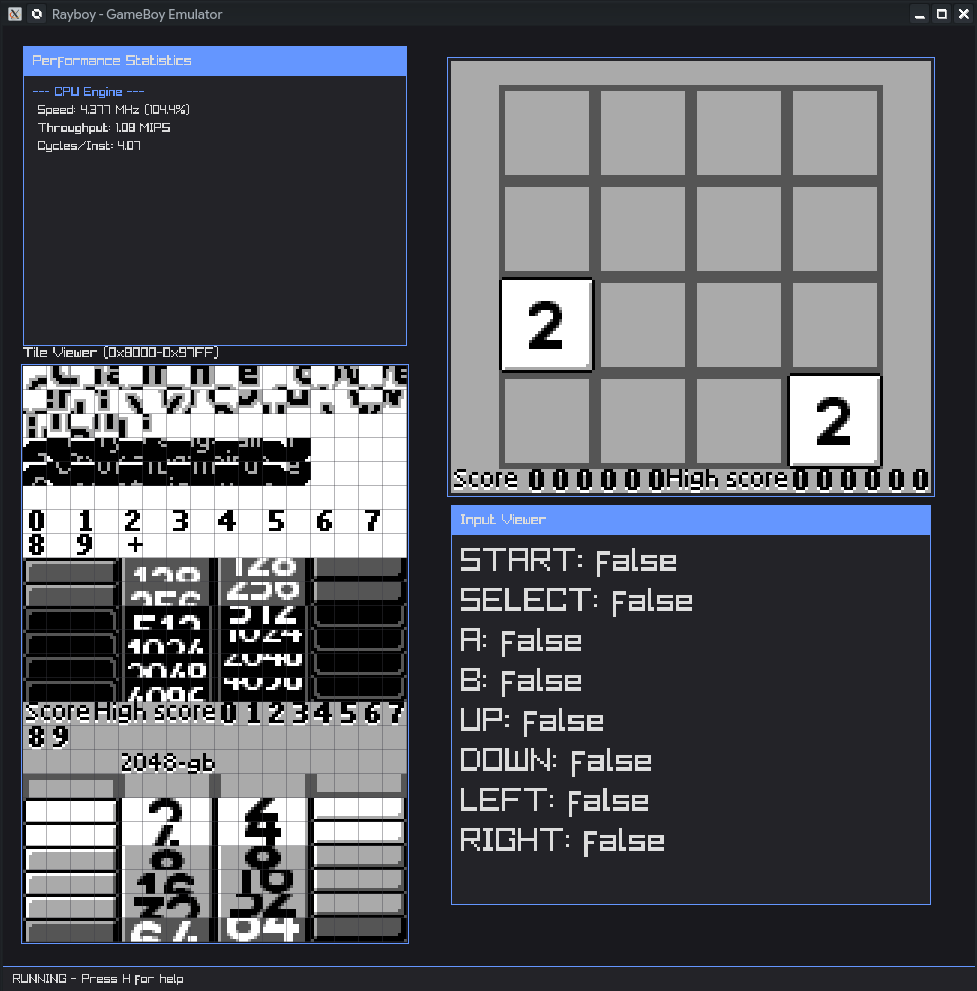
\includegraphics[width=0.9\linewidth]{rayboy_ui.png}
		\caption{Okno emulatora. Źródło: Własnoręczna implementacja}
		\label{fig:rayboy_ui}
	\end{minipage}
\end{figure}


Klasa \texttt{RayboyUI} zarządza wszystkimi elementami graficznymi interfejsu użytkownika. 
Przechowuje ona wskaźnik do struktury współdzielonej \texttt{EmulatorShared}, która 
umożliwia wymianę danych pomiędzy rdzeniem emulatora a warstwą graficzną. 
Struktura ta zawiera między innymi:

\begin{itemize}
	\item bufor klatek obrazu generowanych przez emulator,
	\item dane graficzne kafelków zapisanych w pamięci wideo,
	\item statystyki pracy procesora emulowanego systemu,
	\item flagi sterujące stanem emulatora (np. pauza lub zakończenie pracy).
\end{itemize}

Klasa przechowuje również zmienne opisujące aktualny stan interfejsu, takie jak 
widoczność poszczególnych paneli, w tym podglądu kafelków graficznych, panelu 
statystyk oraz ekranu pomocy.

Dodatkowo zdefiniowane zostały stałe określające parametry wyświetlania, takie jak 
rozdzielczość ekranu oryginalnej konsoli Game Boy (160$\times$144 piksele), 
współczynnik skalowania obrazu oraz liczba wyświetlanych kafelków w podglądzie pamięci 
graficznej.
\subsubsection{Główna pętla interfejsu}

Działanie interfejsu użytkownika opiera się na dwóch podstawowych metodach: 
\texttt{update()} oraz \texttt{draw()}.

Metoda \texttt{update()} odpowiada za aktualizację stanu interfejsu, w tym 
obsługę wejścia użytkownika oraz aktualizację danych graficznych. 
Natomiast metoda \texttt{draw()} realizuje renderowanie wszystkich elementów 
interfejsu, takich jak ekran emulatora, panel statystyk, podgląd kafelków 
oraz pasek statusu.
\subsubsection{Inicjalizacja interfejsu}

Proces inicjalizacji interfejsu realizowany jest przez metodę \texttt{setup()}. 
W trakcie jej wykonywania obliczane są wymiary okna aplikacji na podstawie 
rozmiarów poszczególnych paneli interfejsu. Następnie wyznaczane są pozycje 
elementów graficznych, takich jak panel statystyk, podgląd kafelków oraz ekran 
emulatora.

Kolejnym krokiem jest utworzenie okna aplikacji oraz ustawienie docelowej liczby 
klatek na sekundę. Następnie tworzone są struktury danych typu \texttt{Image} 
oraz \texttt{Texture2D}, które przechowują obraz ekranu emulatora oraz dane 
graficzne podglądu kafelków. Obrazy te są następnie przesyłane do pamięci karty 
graficznej w postaci tekstur, co umożliwia ich szybkie renderowanie.

\subsubsection{Aktualizacja obrazu ekranu}

Aktualizacja obrazu wyświetlanego przez emulator realizowana jest w metodzie 
\texttt{updateScreenTexture()}. W pierwszej kolejności sprawdzana jest flaga 
\texttt{frame\_ready}, która informuje o dostępności nowej klatki obrazu 
wygenerowanej przez rdzeń emulatora.

W przypadku dostępności nowej klatki wykonywane są następujące operacje:

\begin{enumerate}
	\item odczyt indeksu bufora zawierającego aktualną klatkę obrazu,
	\item skopiowanie danych pikseli do lokalnego obrazu interfejsu,
	\item aktualizacja tekstury znajdującej się w pamięci karty graficznej,
	\item wyzerowanie flagi informującej o gotowości klatki.
\end{enumerate}

Zastosowanie takiego mechanizmu pozwala na bezpieczną komunikację pomiędzy 
wątkiem emulatora a wątkiem odpowiedzialnym za renderowanie interfejsu użytkownika.
\newpage
\subsubsection{Renderowanie obrazu emulatora}

\begin{figure}[htbp]
	\centering
	\begin{minipage}{0.65\textwidth}
		\centering
		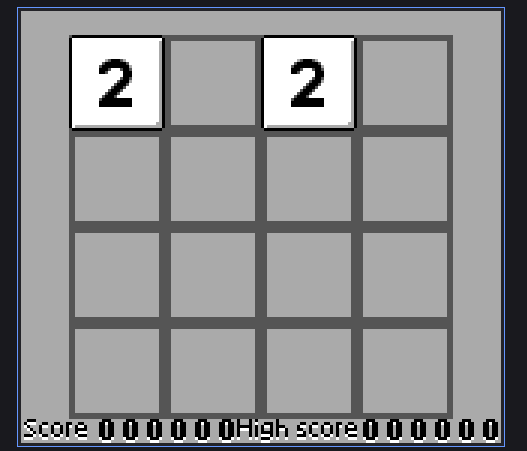
\includegraphics[width=0.9\linewidth]{screen.png}
		\caption{Zrzut emulowanego ekranu. Źródło: Własnoręczna implementacja}
		\label{fig:gameboy_screen}
	\end{minipage}
\end{figure}

Wyświetlanie obrazu generowanego przez emulator realizowane jest w metodzie 
\texttt{drawScreen()}. W pierwszej kolejności rysowana jest ramka otaczająca 
ekran emulatora. Następnie wyświetlana jest tekstura zawierająca aktualną klatkę 
obrazu.

Ponieważ rozdzielczość oryginalnej konsoli Game Boy jest stosunkowo niewielka, 
obraz jest skalowany podczas renderowania. Dzięki temu możliwe jest jego 
czytelne wyświetlenie na ekranie komputera

\subsubsection{Obsługa wejścia użytkownika}
\begin{figure}[htbp]
	\centering
	\begin{minipage}{0.65\textwidth}
		\centering
		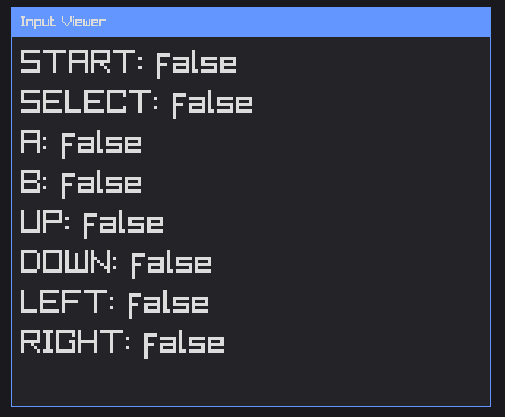
\includegraphics[width=0.9\linewidth]{input_viewer.png}
		\caption{Okienko stanu wirtualnych urządeń wejścia konsoli. Źródło: Własnoręczna implementacja}
		\label{fig:input_viewer}
	\end{minipage}
\end{figure}
Obsługa wejścia z klawiatury realizowana jest w metodzie \texttt{handleInput()}. 
W metodzie tej zdefiniowano zestaw skrótów klawiszowych umożliwiających sterowanie 
pracą emulatora.

Do najważniejszych funkcji należą:

\begin{itemize}
	\item wstrzymanie lub wznowienie emulacji,
	\item zakończenie działania programu,
	\item włączenie lub wyłączenie panelu statystyk,
	\item włączenie lub wyłączenie podglądu kafelków,
	\item wyświetlenie ekranu pomocy.
\end{itemize}

Dodatkowo klawisze klawiatury mapowane są na przyciski kontrolera konsoli Game Boy. 
Stan przycisków zapisywany jest w strukturze \texttt{gamepad\_state}, która 
następnie przekazywana jest do rdzenia emulatora.

\subsubsection{Podgląd kafelków graficznych}
\begin{figure}[htbp]
	\centering
	\begin{minipage}{0.65\textwidth}
		\centering
		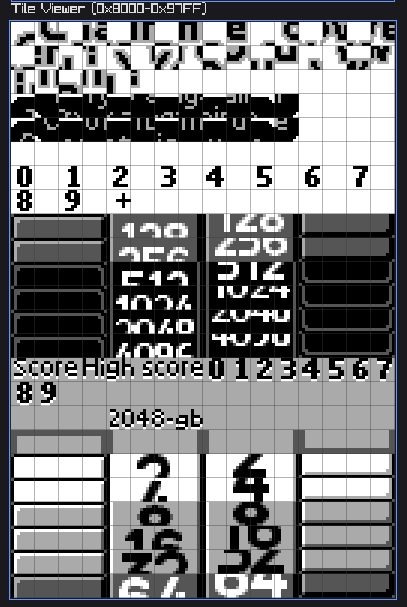
\includegraphics[width=0.9\linewidth]{tile_viewer.png}
		\caption{Podgląd kafelków przechowywanych w pamięci VRAM. Źródło: Własnoręczna implementacja}
		\label{fig:tile_viewer}
	\end{minipage}
\end{figure}
Konsola Game Boy wykorzystuje system grafiki oparty na tzw. kafelkach 
(\textit{tiles}), które są niewielkimi obrazami o rozmiarze 8$\times$8 pikseli. 
Metoda \texttt{updateTileImage()} odpowiada za generowanie obrazu zawierającego 
podgląd wszystkich kafelków zapisanych w pamięci graficznej emulatora.

Dla każdego kafelka wywoływana jest funkcja \texttt{renderTile()}, która 
odczytuje dane pikseli z pamięci wideo, oblicza identyfikator koloru dla 
poszczególnych pikseli oraz rysuje je w odpowiednim miejscu obrazu podglądu.

Podgląd ten jest następnie wyświetlany w interfejsie przy użyciu metody 
\texttt{drawTileViewer()}, która dodatkowo rysuje siatkę ułatwiającą 
identyfikację poszczególnych kafelków.

\subsubsection{Panel statystyk}

\begin{figure}[htbp]
	\centering
	\begin{minipage}{0.65\textwidth}
		\centering
		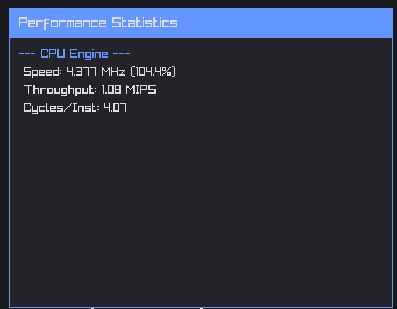
\includegraphics[width=0.9\linewidth]{performance.png}
		\caption{Okienko statystyk emulacji. Źródło: Własnoręczna implementacja}
		\label{fig:perfomance_viewer}
	\end{minipage}
\end{figure}


Interfejs zawiera również panel statystyk wydajności emulatora, który 
wyświetlany jest przez metodę \texttt{drawStatsPanel()}. Panel ten prezentuje 
informacje dotyczące pracy rdzenia emulatora, takie jak:

\begin{itemize}
	\item aktualna prędkość emulowanego procesora wyrażona w MHz,
	\item procentowa zgodność prędkości z oryginalnym sprzętem,
	\item liczba wykonywanych instrukcji na sekundę (MIPS),
	\item średnia liczba cykli procesora przypadających na jedną instrukcję.
\end{itemize}

Informacje te są pomocne podczas analizy wydajności implementacji emulatora 
oraz w procesie jego optymalizacji.

\subsubsection{Ekran Pomocy}

\begin{figure}[htbp]
	\centering
	\begin{minipage}{0.65\textwidth}
		\centering
		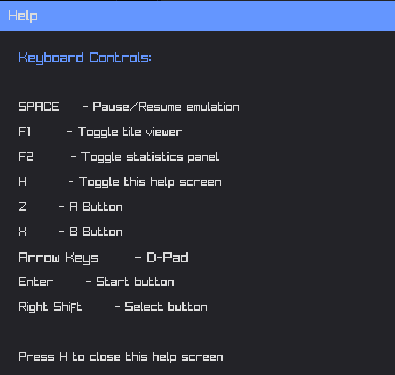
\includegraphics[width=0.9\linewidth]{help_screen.png}
		\caption{Ekran pomocy. Źródło: Własnoręczna implementacja}
		\label{fig:help_screen}
	\end{minipage}
\end{figure}

\subsubsection{Podsumowanie}

Klasa \texttt{RayboyUI} stanowi warstwę prezentacji emulatora i pełni rolę 
pośrednika pomiędzy użytkownikiem a rdzeniem systemu emulacji. 
Odpowiada ona zarówno za wizualizację obrazu generowanego przez emulator, 
jak i za obsługę wejścia użytkownika oraz prezentację informacji 
diagnostycznych. Zastosowanie biblioteki raylib pozwoliło na stosunkowo 
prostą implementację graficznego interfejsu użytkownika przy jednoczesnym 
zachowaniu dobrej wydajności renderowania.

\subsection{Weryfikacja implementacji emulatora}


Weryfikacja implementacji emulatora ma na celu potwierdzenie poprawności odwzorowania zachowania oryginalnego sprzętu. Ze względu na złożoność architektury konsoli Game Boy oraz dużą liczbę zależności pomiędzy jej komponentami, nawet niewielkie odstępstwa od specyfikacji mogą prowadzić do niepoprawnego działania uruchamianych programów. W procesie weryfikacji zastosowano zestaw testów diagnostycznych oraz porównania z referencyjnymi implementacjami emulatorów.

\subsubsection{Metodyka weryfikacji}

Proces weryfikacji opiera się na trzech komplementarnych podejściach. Pierwszym z nich są automatyczne testy diagnostyczne sprawdzające poprawność implementacji podstawowych elementów architektury, takich jak zestaw instrukcji procesora, obsługa przerwań oraz działanie timerów. Drugim etapem jest analiza szczegółowych logów wykonywania programu w przypadku wykrycia niezgodności w działaniu emulatora. Trzecim elementem weryfikacji jest uruchamianie rzeczywistych programów przeznaczonych dla platformy Game Boy oraz porównanie ich działania z referencyjnym emulatorem.

Takie podejście pozwala na weryfikację zarówno niskopoziomowych mechanizmów sprzętowych, jak i poprawności działania emulatora z punktu widzenia użytkownika końcowego.

\subsubsection{Narzędzia testowe}

Podstawowym zestawem testów wykorzystanym w procesie weryfikacji były testy autorstwa \textit{blargg}\cite{blargg}. Zestaw ten jest szeroko stosowany w społeczności twórców emulatorów i służy do sprawdzania poprawności implementacji procesora oraz wybranych elementów sprzętowych konsoli. Testy te weryfikują między innymi działanie instrukcji procesora, obsługę przerwań oraz funkcjonowanie timerów.


\begin{figure}[htbp]
	\centering
	\begin{minipage}{0.45\textwidth}
		\centering
		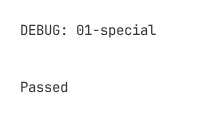
\includegraphics[width=0.9\linewidth]{passed_test.png}
		\caption{Wynik przechodzącego poprawnie testu \textit{01-special.gb}. Własnoręczny zrzut ekranu}
		\label{fig:succesful_blaarg}
	\end{minipage}
\end{figure}


W przypadku niepowodzenia testów przeprowadzana jest dodatkowa analiza przy użyciu narzędzia \textit{gameboy-doctor}\cite{gameboy-doctor}. Emulator generuje plik zawierający szczegółowe logi wykonywania programu, obejmujące stan procesora dla każdego cyklu pracy, w tym wartości rejestrów oraz aktualnie wykonywaną instrukcję.
\begin{figure}[htbp]
	\centering
	\begin{minipage}{0.45\textwidth}
		\centering
		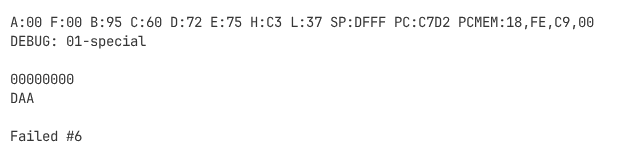
\includegraphics[width=0.9\linewidth]{failed-blaarg.png}
		\caption{Zrzut terminalu z źle zaimplementowanej instrukcji. Własnoręczny zrzut ekranu}
		\label{fig:failed_blaarg}
	\end{minipage}
	\hfill
	\begin{minipage}{0.45\textwidth}
		\centering
		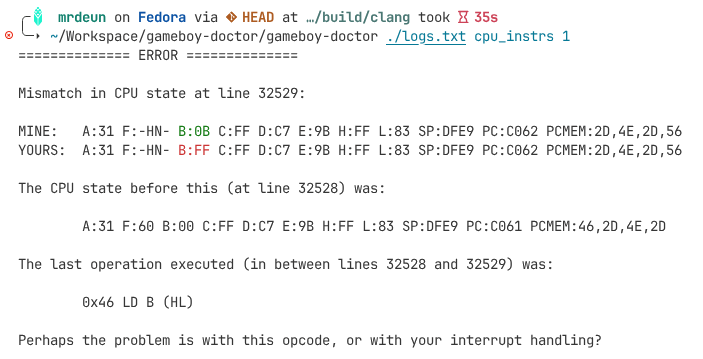
\includegraphics[width=0.9\linewidth]{doctor-gameboy-diagnosis.png}
		\caption{Przykład diagnozy w którym gameboy-doctor wykazał niezgodność procesora. Własnoręczny zrzut ekranu}
		\label{fig:gameboy_doctor}
	\end{minipage}
\end{figure}

 Wygenerowany plik jest następnie przekazywany do narzędzia \textit{gameboy-doctor}, które porównuje go z referencyjnymi logami uzyskanymi z poprawnie działającego emulatora. Narzędzie identyfikuje pierwszy moment, w którym stan procesora zaczyna odbiegać od wartości oczekiwanych, co umożliwia precyzyjne zlokalizowanie błędu w implementacji.

\subsubsection{Testy porównawcze}

Ostatnim etapem weryfikacji było porównanie działania emulatora z dojrzałą implementacją referencyjną. W tym celu wykorzystano emulator \textit{SameBoy}\cite{sameboy}, który jest uznawany za jedną z najbardziej dokładnych implementacji emulatora konsoli Game Boy. 

Porównanie polegało na uruchomieniu tej samej aplikacji typu homebrew w obu emulatorach. Jako program testowy wykorzystano implementację gry \textit{2048}\cite{2048.gb}. Analizie poddano poprawność działania logiki gry, sposób renderowania grafiki oraz reakcję programu na dane wejściowe użytkownika. Zgodność zachowania aplikacji w obu emulatorach stanowi dodatkowe potwierdzenie poprawności implementacji.
\subsection{Problemy implementacyjne}

Przedstawiona implementacja tablicy instrukcji wykorzystuje dwie niestandardowe konstrukcje językowe,
które nie są powszechnie wspierane przez kompilatory C++.

Pierwszą z nich są \textit{designated initializers} (oznaczone inicjalizatory pól struktury),
wprowadzone oficjalnie w standardzie C++20~\cite{cpp20standard}:

\begin{lstlisting}[style=cpp, caption={Oznaczone inicjalizatory pól struktury}]
	vec2 v = {.x = 12.0, .y = 0.3};
\end{lstlisting}

Drugą konstrukcją są \textit{designated initializers} dla tablic, zaczerpnięte z języka C99,
lecz nieuwzględnione w żadnym standardzie C++:

\begin{lstlisting}[style=cpp, caption={Nieoznaczone inicjalizatory tablic -- rozszerzenie niestandardowe}]
	vec2 res[5] = {
		[2] = {.x = 12.0, .y = 0.3},
	};
\end{lstlisting}

O ile oznaczone inicjalizatory pól są obsługiwane przez większość nowoczesnych kompilatorów
zgodnych z C++20, o tyle inicjalizatory indeksowane dla tablic stanowią rozszerzenie
niestandardowe. Aktualnie jedynym kompilatorem C++ obsługującym tę składnię jest
\texttt{clang++}. Kompilatory \texttt{g++} oraz \texttt{MSVC} odrzucają ten kod nawet
przy włączonym standardzie C++23.

Konsekwencją powyższego jest ograniczona przenośność kodu -- projekt można zbudować
wyłącznie przy użyciu \texttt{clang++}, co należy jawnie zaznaczyć w systemie budowania,
na przykład wymuszając wybór kompilatora w pliku \texttt{CMakeLists.txt}:

\begin{lstlisting}[style=cpp, caption={Wymuszenie kompilatora \texttt{clang++} w CMake}]
	set(CMAKE_CXX_COMPILER "clang++" CACHE STRING "" FORCE)
\end{lstlisting}
\newpage
\section{Działanie programu}
\subsection{Struktura Programu}

Kompilacja projektu zwraca plik wykonywalny który należy uruchomić z poziomu terminalu - to uruchomienia pliku gry w emulatorze, należy dać jako argument ścieżke do ROMu \textit{np. ./Rayboy ./2048.gb}.

\subsection{Sterowanie w trakcji działania emulatora}

\begin{itemize}
	\item Kontrola konsoli
	\begin{itemize}
		\item Góra - Strzałka w góre
		\item Dół - Strzałka w dół
		\item Lewo - Strzałka w lewo
		\item Prawo - Strzałka w prawo
		\item START - Enter
		\item SELECT - Prawy Shift
		\item B - B
		\item A - A
	\end{itemize}
	\item Kontrola interfejsu emulatora
	\begin{itemize}
	\item Wszytrzymanie/Wznowienie emulacji - Spacja
	\item Przełączenie widoku na kafelki - 	F1
	\item  Przełączenie widoku statystyk emulatora - F2
	\item Przełączenie ekranu pomocy - H
	\end{itemize}
\end{itemize}
\newpage
\section{Zakończenie}

Celem niniejszej pracy było zaprojektowanie oraz implementacja emulatora konsoli Game Boy. Realizacja tego zadania pozwoliła na praktyczne poznanie wielu zagadnień związanych z architekturą systemów komputerowych, w szczególności z działaniem procesorów oraz sposobem wykonywania instrukcji na niskim poziomie abstrakcji. Implementacja jednostki centralnej emulatora wymagała dokładnego zrozumienia zestawu instrukcji procesora oraz mechanizmu ich interpretacji i wykonywania w środowisku programowym.

Istotnym elementem projektu było również odtworzenie sposobu generowania obrazu przez oryginalny sprzęt. Implementacja części graficznej pozwoliła lepiej zrozumieć, w jaki sposób dane graficzne są przechowywane w pamięci oraz jak są interpretowane przez układ graficzny w celu wygenerowania obrazu na ekranie. Proces ten wymagał odwzorowania specyficznych mechanizmów działania sprzętu oraz odpowiedniej synchronizacji pomiędzy komponentami emulatora.

W trakcie realizacji projektu szczególnie istotną rolę odegrało testowanie poprawności działania emulatora. Ze względu na złożoność emulowanego systemu konieczne było porównywanie zachowania implementacji z rezultatami uzyskiwanymi przez sprawdzone i poprawnie działające emulatory. Tego rodzaju weryfikacja pozwalała na identyfikację błędów oraz stopniowe zwiększanie zgodności implementacji z zachowaniem oryginalnego sprzętu.

Obecna wersja emulatora obsługuje jedynie najprostszy typ kartridża, czyli ROM only. W przyszłości projekt wymaga rozszerzenia o obsługę innych typów kartridży wykorzystujących kontrolery banków pamięci (Memory Bank Controller). Implementacja tych mechanizmów umożliwiłaby uruchamianie znacznie większej liczby gier oraz zwiększyłaby funkcjonalność emulatora.

Należy również zauważyć, że w obecnej wersji projektu kod zawiera elementy zarówno stylu programowania charakterystycznego dla języka C, jak i dla języka C++. Takie podejście nie jest optymalnym rozwiązaniem z punktu widzenia spójności projektu i w przyszłości powinno zostać zastąpione bardziej jednolitą koncepcją implementacyjną. Refaktoryzacja kodu w kierunku konsekwentnego wykorzystania jednego stylu programowania mogłaby poprawić czytelność, łatwość utrzymania oraz dalszy rozwój projektu.

Podsumowując, realizacja emulatora Game Boy stanowiła wartościowe doświadczenie pozwalające na pogłębienie wiedzy z zakresu architektury komputerów, emulacji sprzętu oraz programowania niskopoziomowego. Jednocześnie projekt pozostawia przestrzeń do dalszego rozwoju, zarówno w zakresie rozszerzenia obsługi sprzętu, jak i poprawy jakości oraz struktury kodu.

\newpage
\printbibliography
\end{document}
